\documentclass[fleqn,11pt, titlepage, french]{article}

\setlength{\parindent}{0pt}
\setlength{\parskip}{1em}

\usepackage[T1]{fontenc}
\usepackage{minted}
\usepackage[utf8]{inputenc}
\usepackage{lmodern}
\usepackage[a4paper]{geometry}
\usepackage[francais]{babel}
\usepackage{subfiles}
\usepackage{tabularx}
\usepackage{url}
\usepackage{xcolor}
\usepackage{multicol}
\usepackage{pbox}
\usepackage[hidelinks]{hyperref}
\usepackage{subcaption}

\usepackage{pdfpages}

\usepackage{tikz}

\usepackage{graphicx}

\usepackage{algorithm}
\usepackage{algorithmic}

\usepackage{array}
\usepackage{amsthm}
\usepackage{amssymb}
\usepackage{amsmath}
\usepackage{bbold}
\theoremstyle{plain}
\newtheorem{thm}{Théorème}
\newtheorem{prop}{Proposition}
\newtheorem{coro}{Corollaire}
\newtheorem{lem}{Lemme}

\theoremstyle{definition}
\newtheorem{defn}{Définition}
\newtheorem{exemple}{Exemple}


\theoremstyle{remark}
\newtheorem{rem}{Remarque}
\newtheorem{exercice}{Exercice}
\newtheorem{quest}{Question}

%% Ensemble usuels 

\newcommand{\rel}{\mathbb{Z}}
\newcommand{\nat}{\mathbb{N}}
\newcommand{\rat}{\mathbb{Q}}
\newcommand{\real}{\mathbb{R}}
\newcommand{\complex}{\mathbb{C}}

\newcommand{\Esp}{\mathbb{E}}

\newcommand{\Z}{\rel}
\newcommand{\N}{\nat}
\newcommand{\Q}{\rat}
\newcommand{\R}{\real}
%\newcommand{\C}{\complex}
\newcommand{\ZZ}[1]{\relmod{#1}}

\newcommand{\unit}{\mathbb{U}}
\newcommand{\relmod}[1]{\rel/#1\rel}
\newcommand{\realcontinous}{\mathcal C \left(\real, \real\right)}

\newcommand{\gradient}{\nabla}

%% Notations ephémères
\newcommand{\Arond}{\mathcal A}
\newcommand{\Brond}{\mathcal B}
\newcommand{\Crond}{\mathcal C}
\newcommand{\Drond}{\mathcal D}
\newcommand{\Erond}{\mathcal E}
\newcommand{\Frond}{\mathcal F}
\newcommand{\Grond}{\mathcal G}
\newcommand{\Hrond}{\mathcal H}
\newcommand{\Irond}{\mathcal I}
\newcommand{\Jrond}{\mathcal J}
\newcommand{\Krond}{\mathcal K}
\newcommand{\Lrond}{\mathcal L}
\newcommand{\Mrond}{\mathcal M}
\newcommand{\Nrond}{\mathcal N}
\newcommand{\Orond}{\mathcal O}
\newcommand{\Prond}{\mathcal P}
\newcommand{\Qrond}{\mathcal Q}
\newcommand{\Rrond}{\mathcal R}
\newcommand{\Srond}{\mathcal S}
\newcommand{\Trond}{\mathcal T}
\newcommand{\Urond}{\mathcal U}
\newcommand{\Vrond}{\mathcal V}
\newcommand{\Wrond}{\mathcal W}
\newcommand{\Xrond}{\mathcal X}
\newcommand{\Yrond}{\mathcal Y}
\newcommand{\Zrond}{\mathcal Z}

\newcommand{\Abf}{\mathbf A}
\newcommand{\Bbf}{\mathbf B}
\newcommand{\Cbf}{\mathbf C}
\newcommand{\Dbf}{\mathbf D}
\newcommand{\Ebf}{\mathbf E}
\newcommand{\Fbf}{\mathbf F}
\newcommand{\Gbf}{\mathbf G}
\newcommand{\Hbf}{\mathbf H}
\newcommand{\Ibf}{\mathbf I}
\newcommand{\Jbf}{\mathbf J}
\newcommand{\Kbf}{\mathbf K}
\newcommand{\Lbf}{\mathbf L}
\newcommand{\Mbf}{\mathbf M}
\newcommand{\Nbf}{\mathbf N}
\newcommand{\Obf}{\mathbf O}
\newcommand{\Pbf}{\mathbf P}
\newcommand{\Qbf}{\mathbf Q}
\newcommand{\Rbf}{\mathbf R}
\newcommand{\Sbf}{\mathbf S}
\newcommand{\Tbf}{\mathbf T}
\newcommand{\Ubf}{\mathbf U}
\newcommand{\Vbf}{\mathbf V}
\newcommand{\Wbf}{\mathbf W}
\newcommand{\Xbf}{\mathbf X}
\newcommand{\Ybf}{\mathbf Y}
\newcommand{\Zbf}{\mathbf Z}


%% Topologie

\newcommand{\Topo}{\mathcal{O}}
\newcommand{\Int}[1]{\mathring{#1}}
\newcommand{\Adh}[1]{\overline{#1}}
\newcommand{\Fr}{\mathit{Fr}}
% Espace métriques
\newcommand{\Bo}{\mathcal{B}}
\newcommand{\Bf}{\bar{\mathcal{B}}}

\newcommand{\vertiii}[1]{{\left\vert\kern-0.25ex\left\vert\kern-0.25ex\left\vert #1 
    \right\vert\kern-0.25ex\right\vert\kern-0.25ex\right\vert}}


\newcommand{\congr}{\equiv}
\newcommand{\Vois}{\mathcal{V}}

\newcommand{\SL}{\mathbf{SL}}
\newcommand{\SO}{\mathbf{SO}}
\newcommand{\Bij}{\mathcal Bij}
\newcommand{\Perm}{\mathfrak{S}}

\newcommand{\dd}{\mathrm d}

\newcommand{\onebb}{1\!\!1}

\newcommand{\parts}[1]{\mathcal{P}\left(#1\right)}

\newcommand{\abs}[1]{\left|#1\right|}
\newcommand{\norm}[1]{\left|\left|#1\right|\right|}


\newcommand{\kev}{$\mathbb{K}$-ev }
\newcommand{\Aut}{\mathcal{A}ut}
\newcommand{\signa}{\epsilon}
\newcommand{\inv}[1]{\frac{1}{#1}}

\newcommand{\ds}{\displaystyle}
\newcommand{\fact}[1]{#1~!}

\newcommand{\card}[1]{\left| #1\right|}
%\newcommand{\card}[1]{\##1}
%\newcommand{\card}[1]{\mathrm{Card}\left(#1\right)}

\newcommand{\set}[1]{\left\{ #1\right\}}
\newcommand{\eng}[1]{\left< #1\right>}
\newcommand{\interclosed}[1]{\left[ #1\right]}
\newcommand{\interopend}[1]{\left] #1 \right[}
\newcommand{\im}{\mathrm{Im}}
\renewcommand{\geq}{\geqslant}
\renewcommand{\leq}{\leqslant}
\renewcommand{\iff}{\Leftrightarrow}

\newcommand{\longto}{\longrightarrow}

\newcommand{\Id}{\mathit{Id}}
\newcommand{\Ind}{\mathbb{1}}

\newcommand{\lpar}{\left(}
\newcommand{\rpar}{\right)}

\newcommand{\follows}{\sim}



%% Graphes

\newcommand{\Ger}{\mathbb G}

%% Proba

\newcommand{\Proba}{\mathbb P}
\newcommand{\1}{\matbb 1}
\newcommand{\Bin}{\mathcal B}

\newcommand{\NP}{\mathcal{NP}}
\newcommand{\PP}{\mathcal{P}}


\title{Adam: A method for stochastic Optimization}
\author{Maxime \textsc{Darrin}}


\begin{document}
	\maketitle
	\tableofcontents

	\newpage
	
	\section{Introduction}
	
	Adam est une méthode originellement proposée par en 2015 par D.P Kingma et J. Lei Ba à la conférence ICLR. C'est une méthode d'optimisation du premier ordre introduisant une méthode de conservation du moment d'inertie (\emph{momentum} en anglais) couplée à un \emph{learning rate} adaptatif.
	
	Il reprend le principe de l'\emph{adaptative learning rate} utilisé par \emph{Adadelta\cite{adadelta}} et \emph{RMSProp\cite{rmsprop}}, c'est à dire qu'il conserve une moyenne temporelle (l'importance du passé diminue exponentiellement avec le temps) du carré des gradients précédemment calculés de sorte à conserve une notion de variance des-dits gradients.
		
	A cela, il ajoute une conservation de l'inertie. Il estime la moyenne des gradients (simples cette fois-ci) précédemment calculés, de même que précédemment en accordant plus d'importance aux observations récentes qu'au passé en faisant diminuer exponentiellement avec le temps l'importance du passé. L'idée est de conserver une notion de moyenne de la pente courante et de continuer à aller "un peu" dans les directions prises dans le passé.
	
	Ces deux propriétés simulent en fait la trajectoire qu'une boule qui roulerait (avec de la friction) sur la surface d'erreur, aurait.
	
	Dans un premier temps 
	
	
	\section{Principes et justification}
	
	\subsection{\emph{Adaptavie learning rate}}
	
	Tout d'abord, on rappelle la méthode \emph{RMS Prop} proposée par Geoff Hinton\cite{rmsprop}. On maintient une estimation de la moyenne des carrés des coordonnées des gradients, c'est à dire de la variance non centrée. Et on l'utilise pour adapter le \emph{learning rate}. Dans la suite on notera $g_t$ le vecteur des gradient calculé au temps $t$ et l'application des carrés se fait coordonnées à coordonnées.
	
	\begin{figure}[H]
		\centering
		\begin{align*}
			E[g^2]_t &= 0.9 E[g^2]_{t-1} + 0.1 g^2_t \\ 
			\theta_{t+1} &= \theta_{t} - \dfrac{\eta}{\sqrt{E[g^2]_t + \epsilon}} g_{t} 
		\end{align*}
		\caption{Mise à jour pour \emph{RMSProp}}
	\end{figure}

	\emph{Adam} reprend ce principe de manière plus générale: pour $\beta_2 \in [0,1]$ , on utilise: \[v_t = \beta_2 v_{t-1} +  (1-\beta_2)g_t^2\] comme estimateur de la variance non centrée des gradients. Cependant cet estimateur est biaisé et il est nécessaire de de le redresser.
	
	On suppose tout d'abord que pour tout tout $t$, $g_t \follows p(g_t)$, des distributions de probabilité inconnues. L'objectif est d'exprimer $\Esp[v_t]$ fonction de $\Esp[g_t^2]$ pour en extraire le biais -- et donc savoir comment le corriger.
	
	Tout d'abord, on note que $v_{t}=\left(1-\beta_{2}\right) \sum_{i=1}^{t} \beta_{2}^{t-i} \cdot g_{i}^{2}$.
	
	On peut alors passer à l'espérance et obtenir
	\begin{align*} 
		\mathbb{E}\left[v_{t}\right] &=\mathbb{E}\left[\left(1-\beta_{2}\right) \sum_{i=1}^{t} \beta_{2}^{t-i} \cdot g_{i}^{2}\right] \\ 
		&=\left(1-\beta_{2}\right) \sum_{i=1}^{t} \beta_{2}^{t-i}  \mathbb{E} [g_{i}^{2}] &\text{Par linéarité de l'espérance} \\ 
		&=\left(1-\beta_{2}\right) \sum_{i=1}^{t} \beta_{2}^{t-i}  (\mathbb{E} [g_{t}^{2}] + \zeta_i)  		&\text{où $\Esp g_{i}^{2} = \Esp[g_{t}^{2}] + \zeta_i$} \\
		&=\left(1-\beta_{2}\right) \sum_{i=1}^{t} (\beta_{2}^{t-i}  \mathbb{E} [g_{t}^{2}] + \beta_{2}^{t-i} \zeta_i) \\
		&=\left(1-\beta_{2}\right) \sum_{i=1}^{t} \beta_{2}^{t-i}  \mathbb{E} [g_{t}^{2}] + \left(1-\beta_{2}\right) \sum_{i=1}^{t} \beta_{2}^{t-i} \zeta_i \\
		&=\mathbb{E}\left[g_{t}^{2}\right] \cdot\left(1-\beta_{2}\right) \sum_{i=1}^{t} \beta_{2}^{t-i}+\zeta \\ 
		&=\mathbb{E}\left[g_{t}^{2}\right] \cdot\left(1-\beta_{2}^{t}\right)+\zeta
	\end{align*}
	
	Le terme $\zeta = \sum_{i=1}^{t} \beta_{2}^{t-i}+\zeta$ est rendu petit en compensant les écarts grandissants entre le dernier gradient et les gradients plus lointains par le poids exponentiellement décroissant qui leurs sont attribués.
	
	Ainsi on note qu'il suffit de diviser notre estimateur par $1-\beta_{2}^{t}$ pour le redresser. On obtient alors l'estimateur proposé pour \emph{Adam} qui est non biaisé.
	\begin{align*}
		\hat{v}_t &= \dfrac{v_t}{1 - \beta^t_2}
	\end{align*}
	
	\subsection{Inertie}
	
	En plus de l'adaptation du \emph{learning rate} \emph{Adam} conserve de l'inertie dans sa descente de gradient, pour ce faire maintien une estimation de la moyenne des prédédents gradients, pour $\beta_1$: $m_t = \beta_1 m_{t-1} + (1-\beta_1) g_t$
	
	De la même manière que pour la variance, cet estimateur est biaisé et on veut le redresser.
	
	\begin{align*} 
	\mathbb{E}\left[m_{t}\right] &=\mathbb{E}\left[\left(1-\beta_{1}\right) \sum_{i=1}^{t} \beta_{1}^{t-i} \cdot g_{i}\right] \\ 
	&=\left(1-\beta_{1}\right) \sum_{i=1}^{t} \beta_{1}^{t-i}  \mathbb{E} [g_{i}] &\text{Par linéarité de l'espérance} \\ 
	&=\left(1-\beta_{1}\right) \sum_{i=1}^{t} \beta_{1}^{t-i}  (\mathbb{E} [g_{t}] + \zeta_i)  		&\text{où $\Esp g_{i} = \Esp[g_{t}] + \zeta_i$} \\
	&=\left(1-\beta_{1}\right) \sum_{i=1}^{t} (\beta_{1}^{t-i}  \mathbb{E} [g_{t}] + \beta_{1}^{t-i} \zeta_i) \\
	&=\left(1-\beta_{1}\right) \sum_{i=1}^{t} \beta_{1}^{t-i}  \mathbb{E} [g_{t}] + \left(1-\beta_{1}\right) \sum_{i=1}^{t} \beta_{1}^{t-i} \zeta_i \\
	&=\mathbb{E}\left[g_{t}\right] \cdot\left(1-\beta_{1}\right) \sum_{i=1}^{t} \beta_{1}^{t-i}+\zeta \\ 
	&=\mathbb{E}\left[g_{t}\right] \cdot\left(1-\beta_{1}^{t}\right)+\zeta
	\end{align*}
	
	De la même façon que pour la variance $\zeta$ est négligeable quitte à choisir une bonne valeur de $\beta_{2}$
	\begin{align*}
		\hat{m}_t &= \dfrac{m_t}{1 - \beta^t_1}
	\end{align*}
	
	\subsection{Couplage des deux grandeurs}
	
	En couplant les estimations de l'inertie et de la variance on obtient une règle de mise à jour qui adapte le \emph{learning rate} et qui simule l'inertie de descente:
	\begin{center}
	$
		\begin{array}{ll}
		m_t = \beta_1 m_{t-1} + (1-\beta_1) g_t & \hat{m}_t = \dfrac{m_t}{1 - \beta^t_1} \\
		v_t = \beta_2 b_{t-1} +  (1-\beta_2)g_t^2 & \hat{v}_t = \dfrac{v_t}{1 - \beta^t_2} \\
		
		\theta_{t+1} = \theta_{t} - \dfrac{\eta}{\sqrt{\hat{v}_t} + \epsilon} \hat{m}_t & \\
		\end{array}
	$
	\end{center}

	On peut alors analyser la règle de mise à jour. On a $\Delta_{t+1} = \theta_{t+1} - \theta_{t} = - \frac{\eta}{\sqrt{\hat{v}_t} + \epsilon} \hat{m}_t$. Ainsi, la taille d'un pas de la descente de gradient est de l'ordre de $\frac{\hat{m}_t}{\sqrt{\hat{v}_t}}$, c'est à dire la moyenne sur le carré de la variance non centrée qui est ici le ratio signal bruit. Et on voit donc, que lorsque ce ratio est faible, c'est à dire que le bruit est élevé -- et donc l'incertitude sur la direction à suivre, on fait des pas plus petits ce qui correspond intuitivement à ce que l'on voudrait faire. En effet, cette incertitude est en général d'autant plus grande qu'on se rapproche d'un minimum (local ou non). Au contraire, lorsque ce ratio est élevé, on peut se permettre de faire de plus grands pas sans risques.
	
	
	
	
	\section{Algorithme ADAM}
	\subsection{Pseudo code}
	\begin{algorithm}[H]
		\begin{algorithmic}
			\REQUIRE{$\eta$ stepsize}
			\REQUIRE{$\beta_1, \beta_2, \epsilon \in  [0,1]$}
			\REQUIRE{$f(\theta)$ loss to minimize}
			
			\STATE{Initialize $\theta_0$}
			\STATE{Initialize $m_0, v_0$ to zeros vectors}
			\STATE{$t \gets 0$}
			
			\WHILE{$\theta_n$ has not converged}
				\STATE{$g_t \gets \gradient_{\theta_t} f(\theta_t)$}
				\STATE{$m_t \gets \beta_1 m_{t-1} + (1-\beta_1) g_t$}
				\STATE{$v_t \gets \beta_2 b_{t-1} +  (1-\beta_2)g_t^2$}
				\STATE{$\hat{m}_t \gets \dfrac{m_t}{1 - \beta^t_1}$}
				\STATE{$ \hat{v}_t \gets \dfrac{v_t}{1 - \beta^t_2}$}
				
				\STATE{$\theta_{t+1} \gets \theta_{t} - \dfrac{\eta}{\sqrt{\hat{v}_t} + \epsilon} \hat{m}_t$}
				\STATE{$t \gets t +1$}
			\ENDWHILE
		\end{algorithmic}
	\caption{Adam}
	\end{algorithm}

	\subsection{Implémentation python}
	
	\begin{figure}[H]
		\centering
\begin{minted}{python}
# Computing adam mean and variance
m = beta1 * prev_m + (1-beta1)*grad
v = beta2 * prev_v + (1-beta2)*np.power(grad, 2)

# We correct them to avoid biais to 0
mchap = m / (1-np.power(beta1, t))
vchap = v / (1-np.power(beta2, t))

# update weights
w = w - (eta / (np.sqrt(vchap)+eps)) * mchap
		\end{minted}
		\caption{Pas de descente de Adam en python}
	\end{figure}

	\subsection{Garanties théoriques}
	
	Les auteurs de \emph{Adam} proposent un résultat de convergence avec une borne sur le regret atteint par l'algorithme. Nous ne donnerons pas ici la preuve en détails car elle est particulièrement longue mais elle est disponible en annexe du papier original\cite{adam}.
	
	On se place dans le cadre décrit par \cite{zinka}. Considérons que nous disposons de $f_1 \cdots f_T$ fonctions de coûts, convexes. A chaque pas de temps on va essayer d'obtenir $\theta_t$ de sorte à minimiser tous les $f_t(\theta_t)$ et on va comparer notre résultat à la solution optimale. On définit ainsi le regret accumulé sur la séquence:
	\[R(T)=\sum_{t=1}^{T}\left[f_{t}\left(\theta_{t}\right)-f_{t}\left(\theta^{*}\right)\right]\]
	
	Avec $\theta^* = \arg\min_{\theta} \sum_{t=1}^T f_t(\theta)$, c'est à dire les paramètres minimisant globalement les $f_t$.
	
	Ce processus correspond à la procédure d'entraînement par \emph{batch} dans laquelle on entraîne le modèle séquentiellement par minimisation de fonctions de coûts définies par le \emph{batch} courant.
	
	Dans le cadre précédent, on suppose que toutes les $f_t$ sont lipschitzienne pour la norme euclidienne et la norme infinie, de constantes respectivement $D$ et $D_\infty$. On suppose de plus que la distance entre deux $\theta$ consécutifs issus de \emph{adam} est bornée pour les deux normes précédentes par $D$ et $D_\infty$ respectivement. Plus clairement, on demande que les pas générés par \emph{adam} soient de longueurs plus petites que les constante de Lipschitz des fonctions de coûts. Par ailleurs, on suppose que $\beta_{1}, \beta_{2}$ ont été choisi de sorte que $\frac{\beta_{1}^{2}}{\sqrt{\beta_{2}}}<1$
	On pose alors $\alpha_{t}=\frac{\alpha}{\sqrt{t}}$ et $ \beta_{1, t}=\beta_{1} \lambda^{t-1}, \lambda \in(0,1)$. 
	
	On note aussi, $g_{1:T, i} = (g_{1,i} \cdots g_{T,i})$, $\gamma = \frac{\beta_1^2}{\sqrt{\beta_2}}$.
	
	On peut alors borner le regret atteint par \emph{Adam}:
	\[R(T) \leq \frac{D^{2}}{2 \alpha\left(1-\beta_{1}\right)} \sum_{i=1}^{d} \sqrt{T \widehat{v}_{T, i}}+\frac{\alpha\left(1+\beta_{1}\right) G_{\infty}}{\left(1-\beta_{1}\right) \sqrt{1-\beta_{2}}(1-\gamma)^{2}} \sum_{i=1}^{d}\left\|g_{1: T, i}\right\|_{2}+\sum_{i=1}^{d} \frac{D_{\infty}^{2} G_{\infty} \sqrt{1-\beta_{2}}}{2 \alpha\left(1-\beta_{1}\right)(1-\lambda)^{2}}\]
	
	Les auteurs notes en particulier que dans le cas où les gradients sont très creux -- par exemple lorsque les données en entrées le sont -- le terme $\sum_{i=1}^{d}\left\|g_{1: T, i}\right\|_{2}$ peut être particulièrement petit et mener à des résultats de convergences plus forts dans certains cas.
	
	Néanmoins, dans le cas général on peut obtenir un regret moyen asymptotique de l'ordre $\Orond(\frac{1}{\sqrt{T}})$. Il suffit d'utiliser dans l'expression précédente le fait que $\sum_{i=1}^{d}\left\|g_{1: T, i}\right\|_{2} \leq d G_\infty \sqrt{T}$, car les gradients sont bornés par hypothèses.
	
	En effet on a:
	\begin{align*}
		R(T) & \leq \frac{D^{2}}{2 \alpha\left(1-\beta_{1}\right)} \sum_{i=1}^{d} \sqrt{T \widehat{v}_{T, i}}+\frac{\alpha\left(1+\beta_{1}\right) G_{\infty}}{\left(1-\beta_{1}\right) \sqrt{1-\beta_{2}}(1-\gamma)^{2}} \sum_{i=1}^{d}\left\|g_{1: T, i}\right\|_{2}+\sum_{i=1}^{d} \frac{D_{\infty}^{2} G_{\infty} \sqrt{1-\beta_{2}}}{2 \alpha\left(1-\beta_{1}\right)(1-\lambda)^{2}} \\
		&\leq \frac{D^{2}}{2 \alpha\left(1-\beta_{1}\right)} \sum_{i=1}^{d} \sqrt{T \widehat{v}_{T, i}}+\frac{\alpha\left(1+\beta_{1}\right) G_{\infty}}{\left(1-\beta_{1}\right) \sqrt{1-\beta_{2}}(1-\gamma)^{2}} d G_\infty \sqrt{T} +\sum_{i=1}^{d} \frac{D_{\infty}^{2} G_{\infty} \sqrt{1-\beta_{2}}}{2 \alpha\left(1-\beta_{1}\right)(1-\lambda)^{2}} \\
		&\underset{T \longrightarrow \infty}{\follows} \frac{D^{2}}{2 \alpha\left(1-\beta_{1}\right)} \sum_{i=1}^{d} \sqrt{T \widehat{v}_{T, i}}+\frac{\alpha\left(1+\beta_{1}\right) G_{\infty}}{\left(1-\beta_{1}\right) \sqrt{1-\beta_{2}}(1-\gamma)^{2}} d G_\infty \sqrt{T} \\
		&\underset{T \longrightarrow \infty}{=} \Orond(\sqrt{T})
	\end{align*}
	D'où $\frac{R(T)}{T} \underset{T \longrightarrow \infty}{=} \Orond(\frac{1}{\sqrt{T}})$

	\section{Résultats empiriques}
	
	\subsection{Comportement sur des problèmes jouets}
	
	On commence par tester l'algorithme présenté pour optimiser des fonctions jouets et on compare les résultats obtenus avec une descente de gradient usuelle. Le problème présenté ici consiste à minimiser la fonction $f_{y_1, y_2} = \norm{x-y_1} * (\norm{x-y_2} +2) $, avec $y_1 = (-10, 0)$ et $y_2 = (10, 0)$. Cette fonction assure la présence de deux minimums locaux en $y_1$ et en $y_2$ avec le minimum global en $y_1$ meilleur que celui en $y_2$. On va utiliser cette dissymétrie pour comparer les différents algorithmes et leur capacité à trouver le minimum global.
	
	Dans les exemples ci-dessous, on observe qu'\emph{Adam} est plus effficace que les autres algorithmes pour trouver le minimum global comme on peut le voir il rejoint toujours le meilleur minimum dans ces exemples. Même placé proche de $y_2$, il arrive à s'extirper de la pente la plus "proche" pour atteindre $y_1$ dans plus de cas que les autres algorithmes.
	
	\begin{figure}[H]
		\centering
		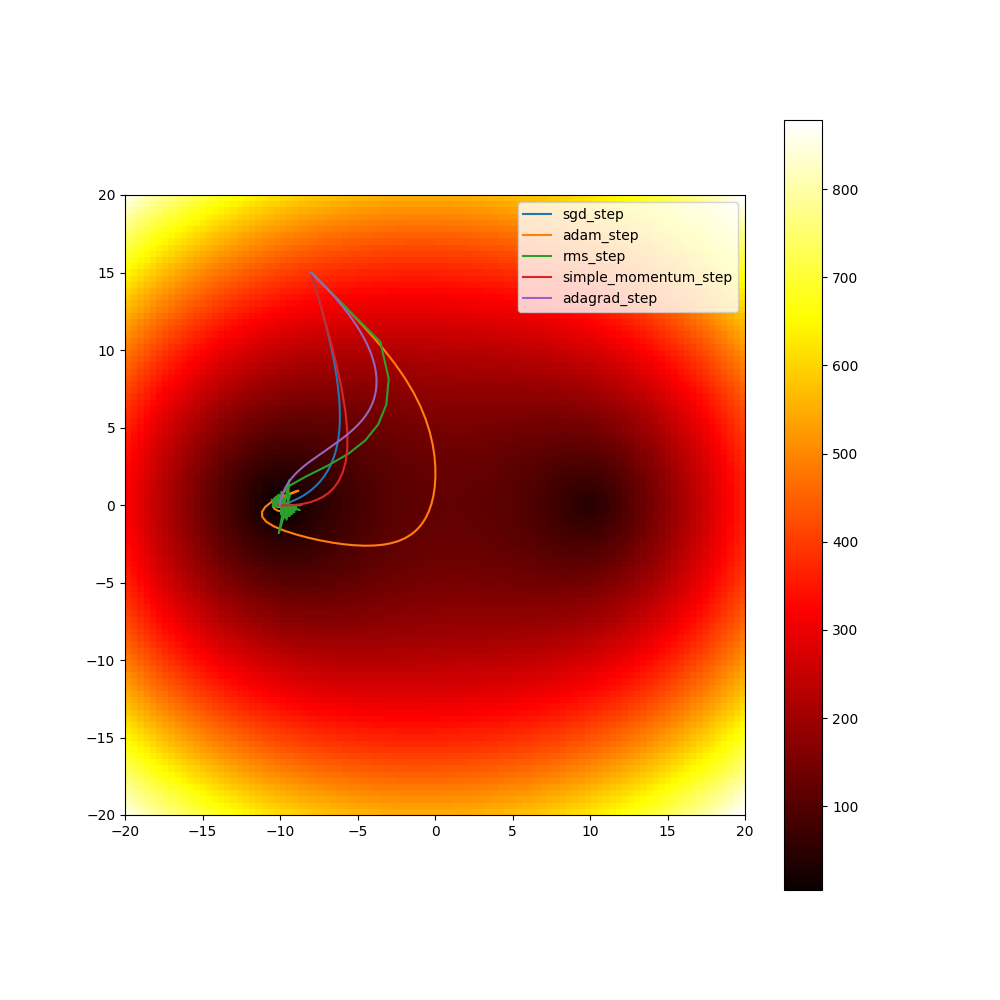
\includegraphics[scale=0.3]{../gdsvm/exports/adam-rms-sgd.png}
		\caption{Comparaison entre adam et différents algorithmes usuels}
	\end{figure}

	\begin{figure}[H]
		\centering
		\begin{subfigure}{0.45\textwidth}
			\centering
			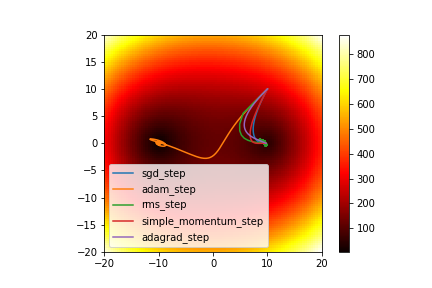
\includegraphics[scale=0.5]{../gdsvm/exports/init-0.png}
		\end{subfigure}
	\begin{subfigure}{0.45\textwidth}
		\centering
		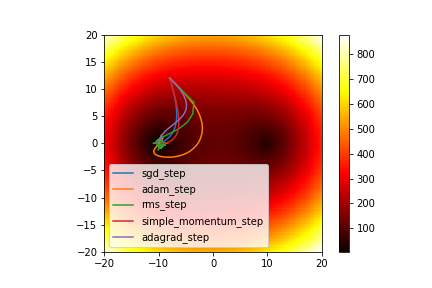
\includegraphics[scale=0.5]{../gdsvm/exports/init-1.png}
	\end{subfigure}
\begin{subfigure}{0.45\textwidth}
	\centering
	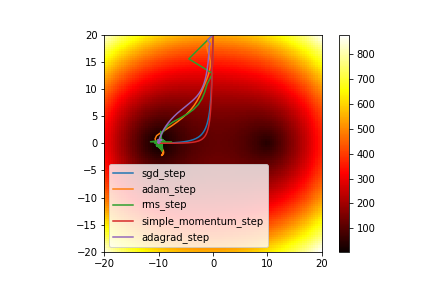
\includegraphics[scale=0.5]{../gdsvm/exports/init-2.png}
\end{subfigure}
\begin{subfigure}{0.45\textwidth}
	\centering
	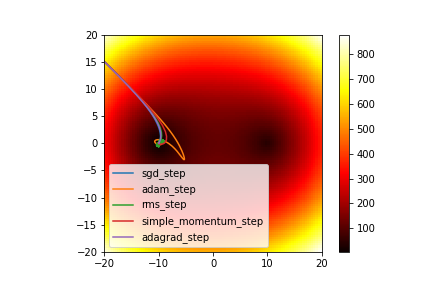
\includegraphics[scale=0.5]{../gdsvm/exports/init-3.png}
\end{subfigure}
\caption{Différentes trajectoires avec différentes initialisations}
	\end{figure}

	
	\subsection{Résultats sur MNIST}
	
	\subsubsection{Protocole expérimental}
	
	On utilise le jeu de données d'entraînement complet pour entraîner par batch la SVM du cours à partir de fonction donnant le gradient de la fonction de coût que l'on souhaite minimiser données en cours.
	
	On effectue un nombre d'epoch fixé et pour chaque epoch on fait une passe sur l'ensemble du jeu de données scindé en batch. Pour chaque batch (et donc pas de descente) on sauvegarde l'erreur courante et la précision courante sur le batch en cours et sur l'ensemble du jeu de test pour constituer les graphiques qui suivent.
	
	\subsubsection{Aperçu global et premières comparaisons}
	
	\begin{figure}[H]
		\centering
		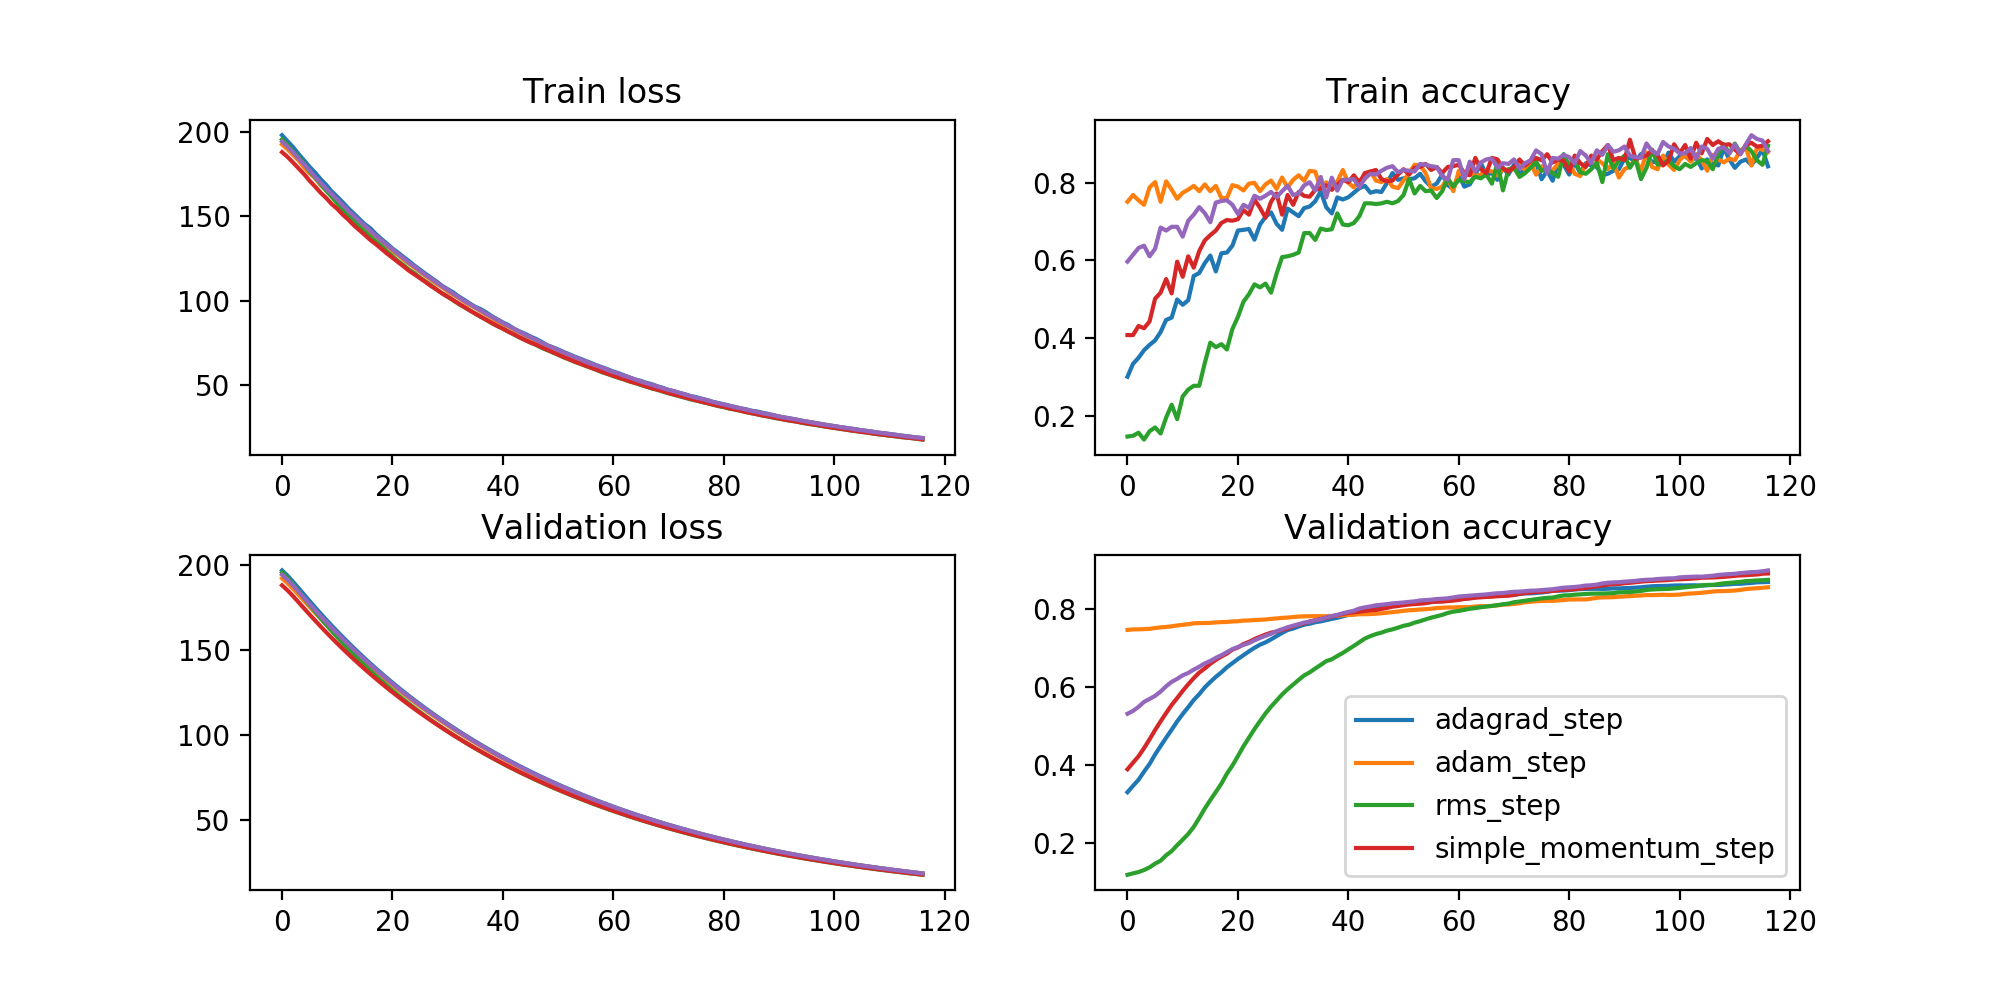
\includegraphics[width=1\linewidth]{../gdsvm/exports/mnist-comparison}
		\caption{Comparaison globale d'Adam sur MNIST}
		\label{fig:mnist-comparison}
	\end{figure}
	
	
		\begin{figure}[H]
		\centering
		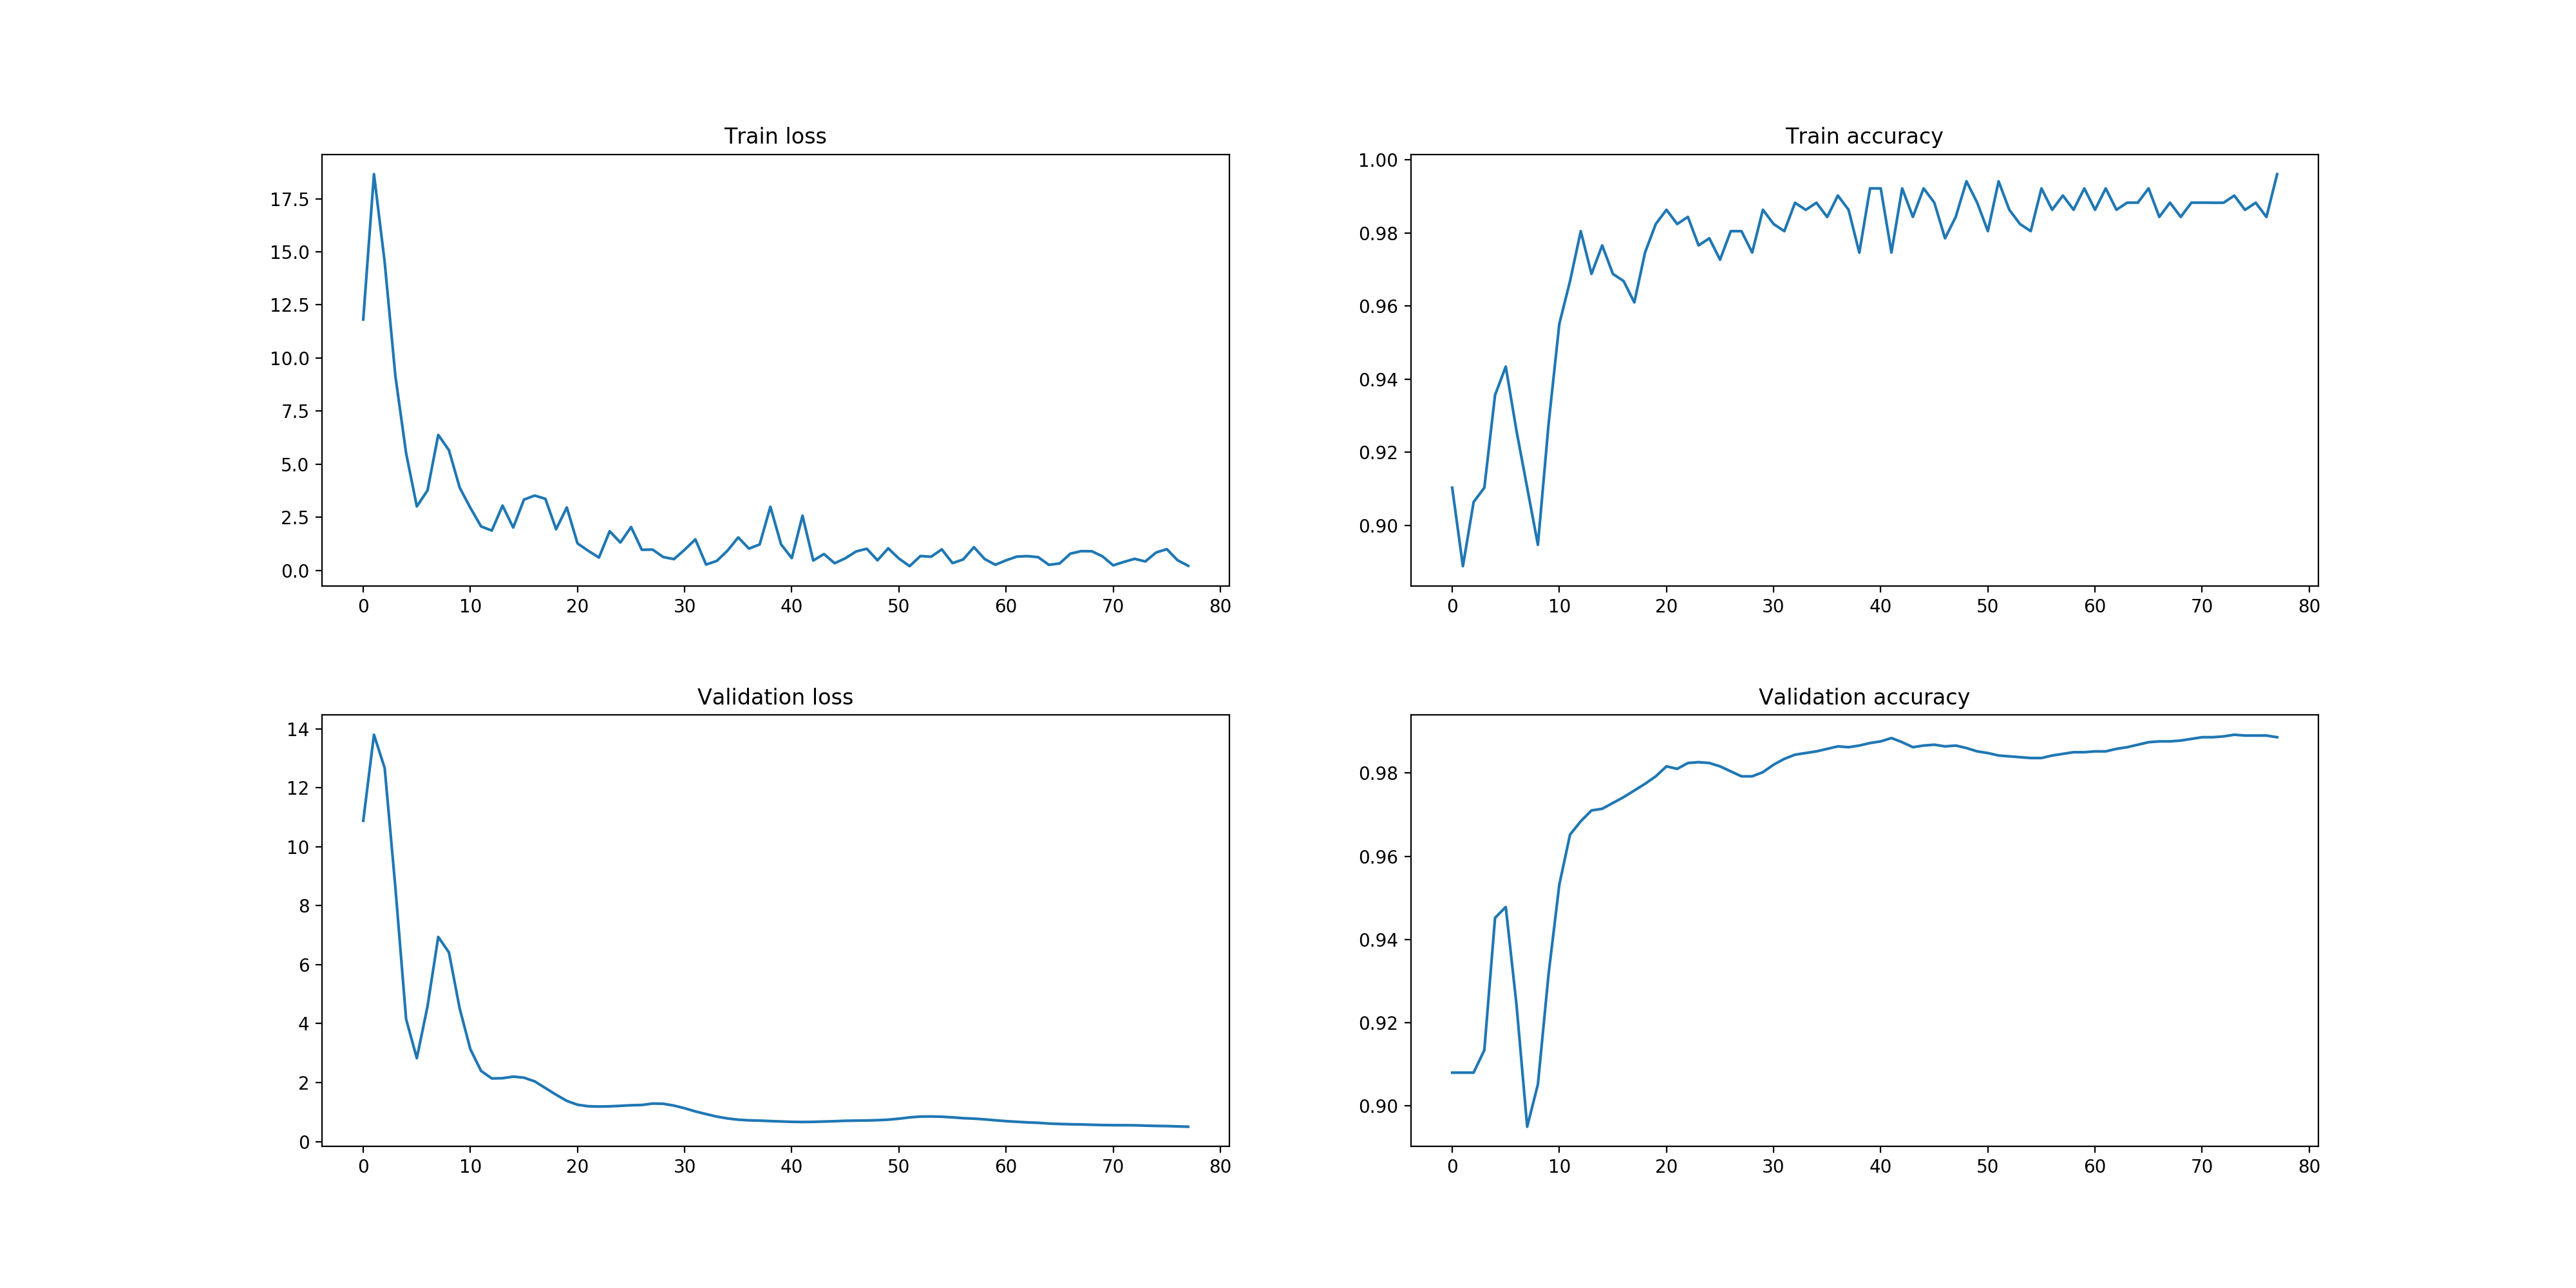
\includegraphics[scale=0.35]{../gdsvm/exports/adam_train.png}
		\caption{Erreur et précision sur MNIST pour le jeu d'entraînement et le jeu de validation}
	\end{figure}
	
	
	\subsubsection{Efficacité de Adam selon la taille des batch}
	
	L'une des motivations avancées pour le développement d'\emph{Adam} par ses auteurs était la résistance à ce genre de bruit induit par les différentes fonctions définies par chaque batch. On peut donc comparer la résilience d'\emph{Adam} face à différentes tailles de batch.
	
	Tout d'abord on peut observer l'influence de la taille des batch sur Adam seul\footnote{Tous les graphes sont disponibles en grande taille dans le dossier gdsvm/exports/.}.
	
	On présente d'abord ici globalement les effets de la taille des batchs sur tous les algorithmes, puis plus précisément l'effet de cette taille sur les très petits batchs.
	
			\begin{figure}[H]
		\centering
		\begin{subfigure}{0.45\textwidth}
			\centering
			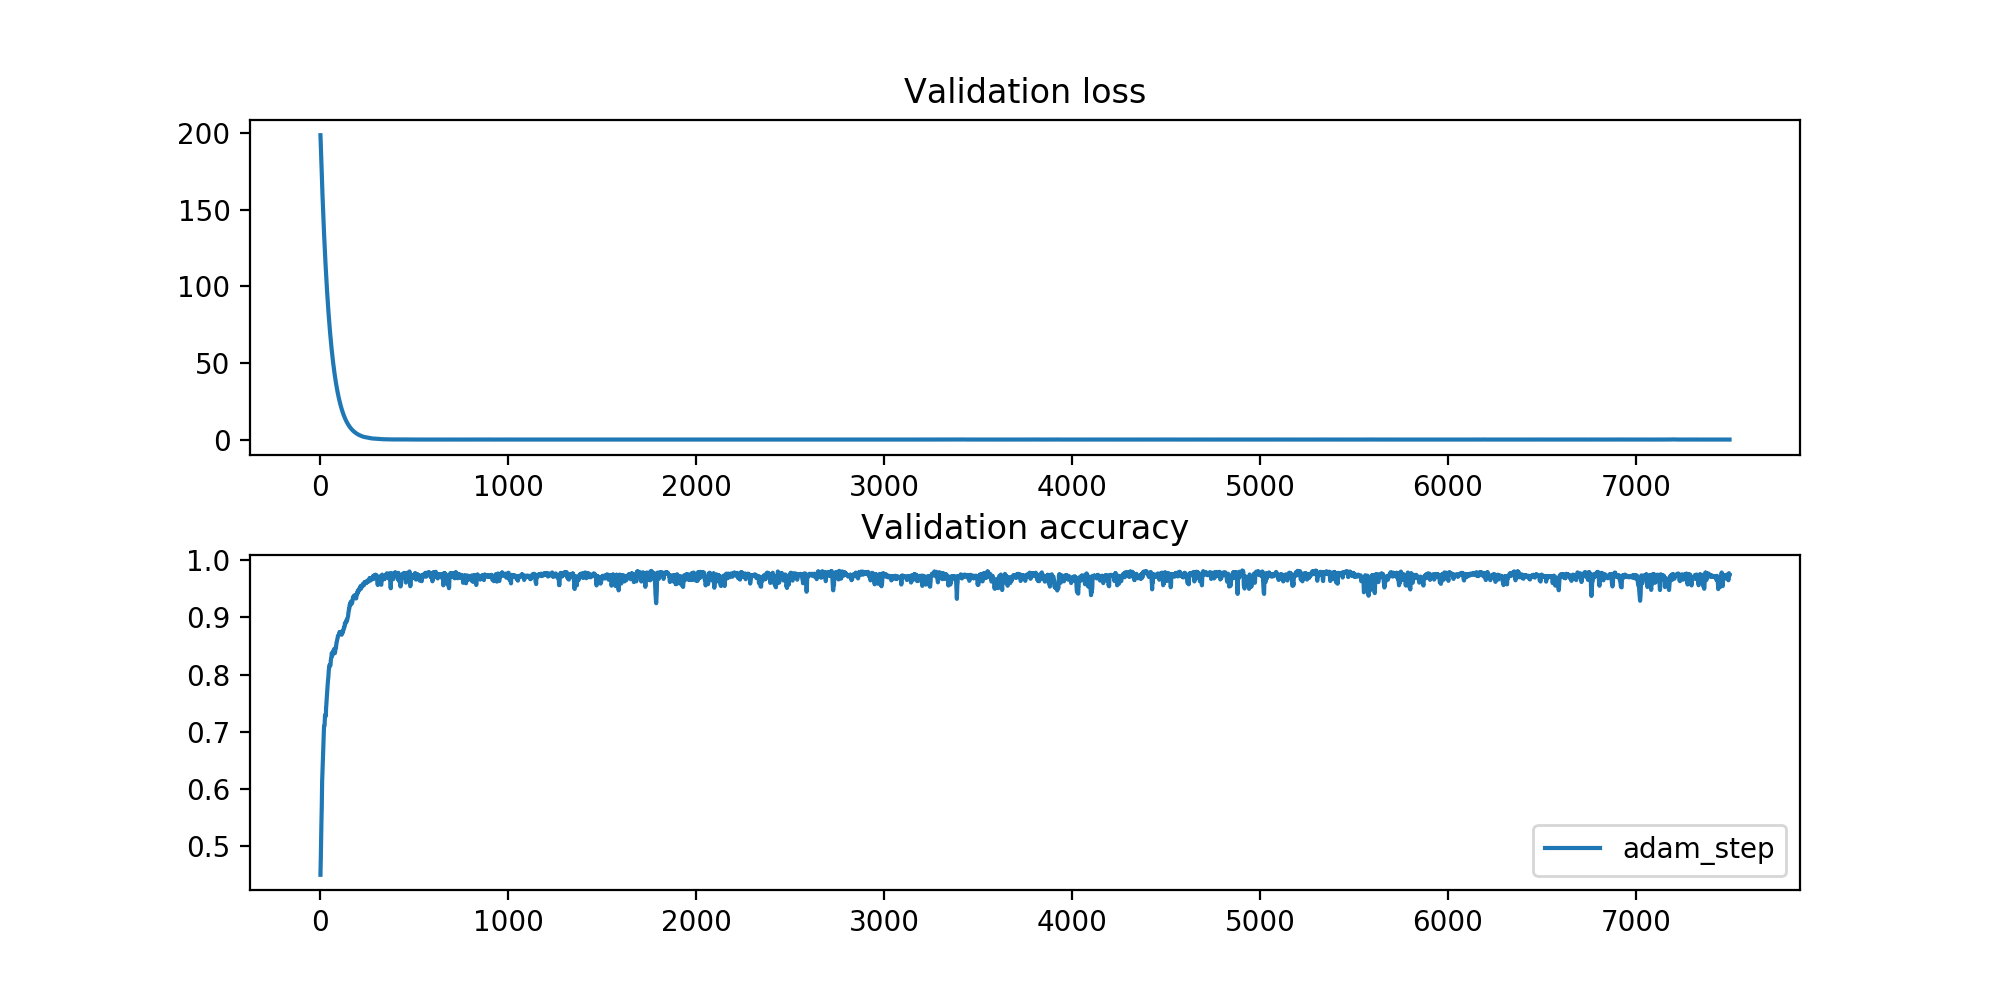
\includegraphics[scale=0.25]{../gdsvm/exports/mnist-batch8-adam_step.png}
			\caption{batch\_size = 8}
		\end{subfigure}
		\begin{subfigure}{0.45\textwidth}
			\centering
			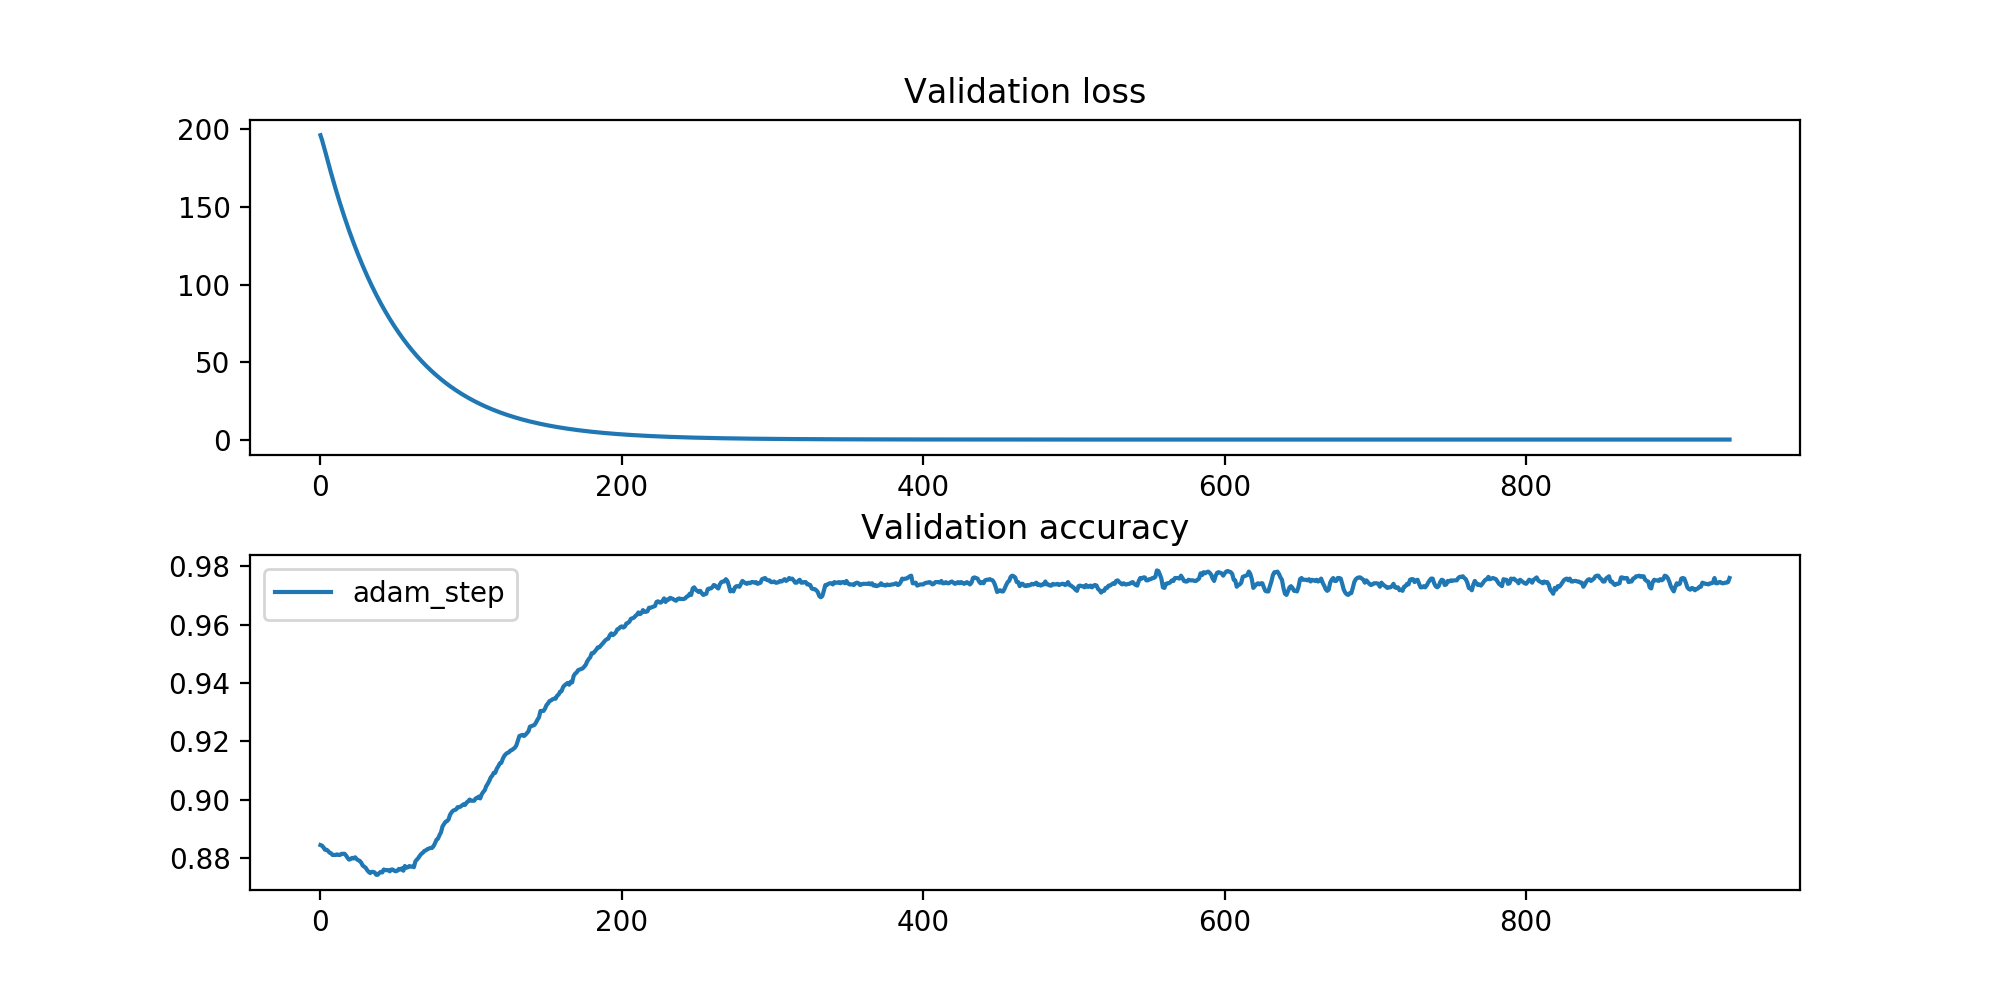
\includegraphics[scale=0.25]{../gdsvm/exports/mnist-batch64-adam_step.png}
			\caption{batch\_size = 64}
		\end{subfigure}
		\begin{subfigure}{0.45\textwidth}
			\centering
			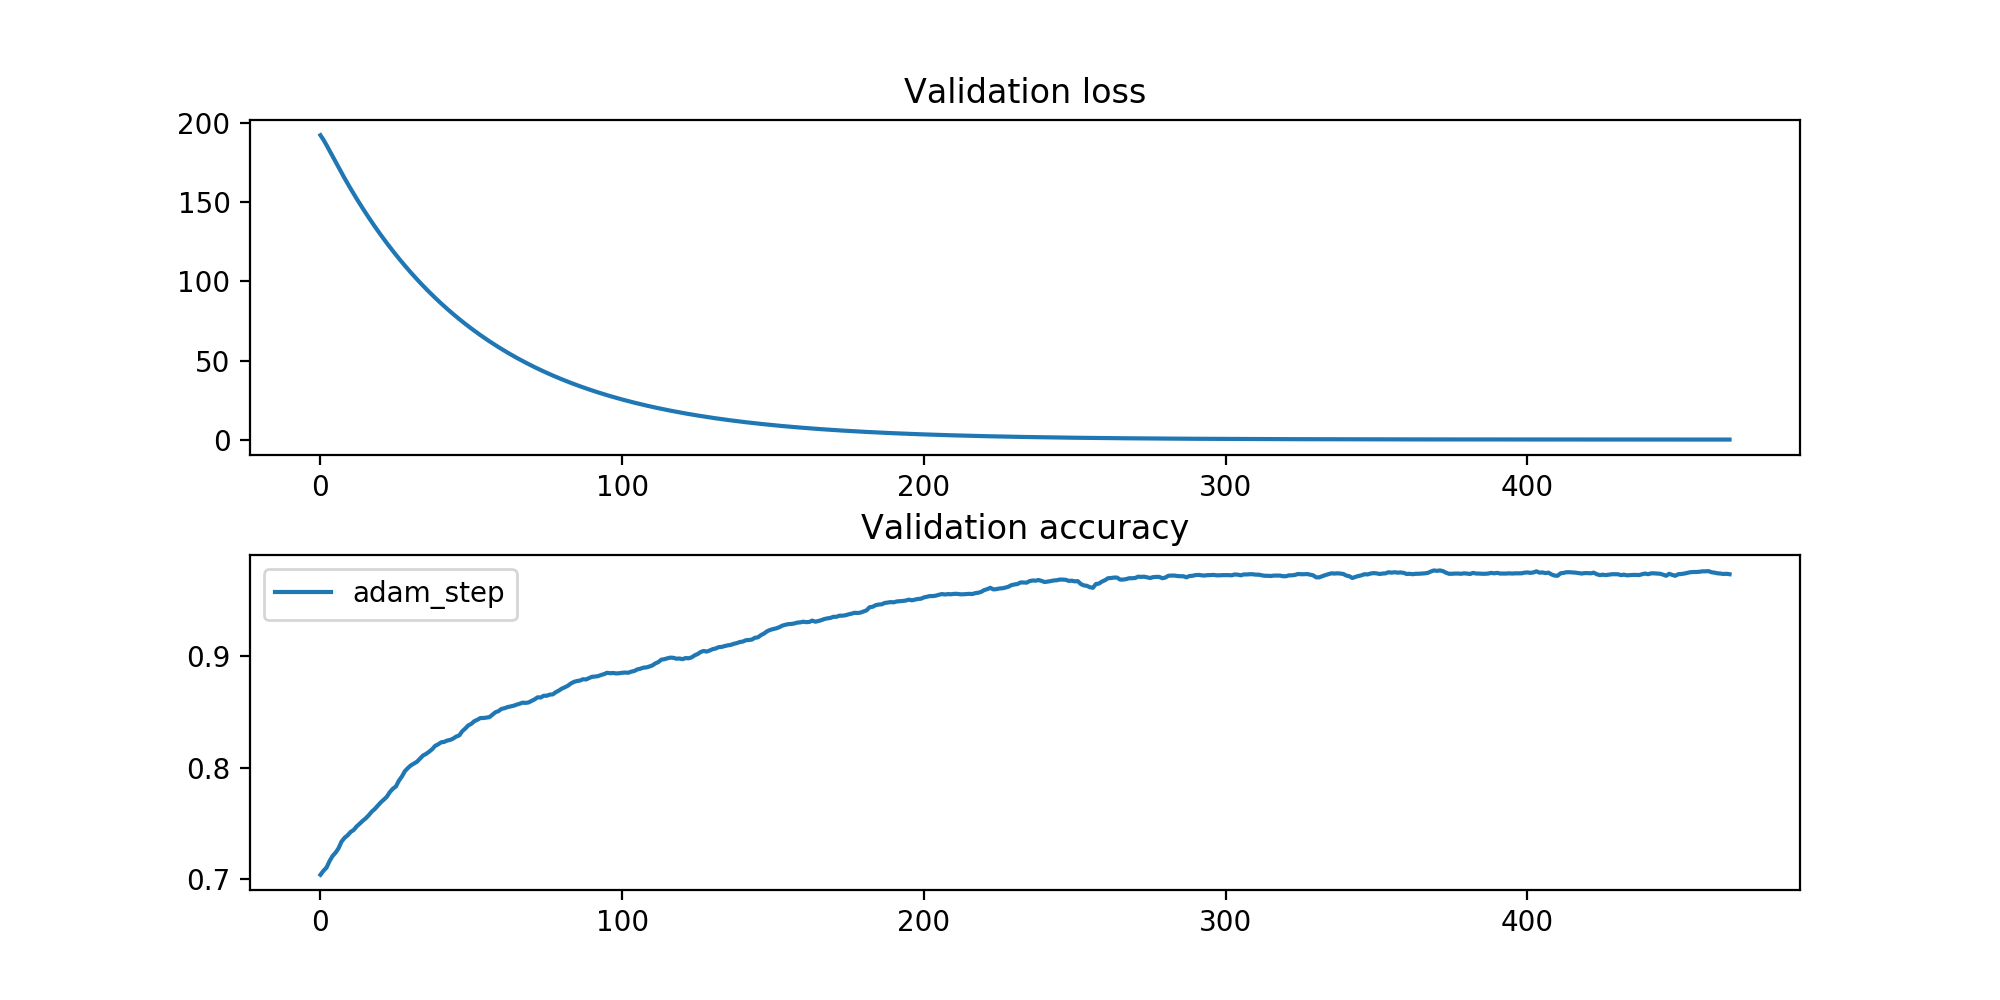
\includegraphics[scale=0.25]{../gdsvm/exports/mnist-batch128-adam_step.png}
			\caption{batch\_size = 128}
		\end{subfigure}
		\begin{subfigure}{0.45\textwidth}
			\centering
			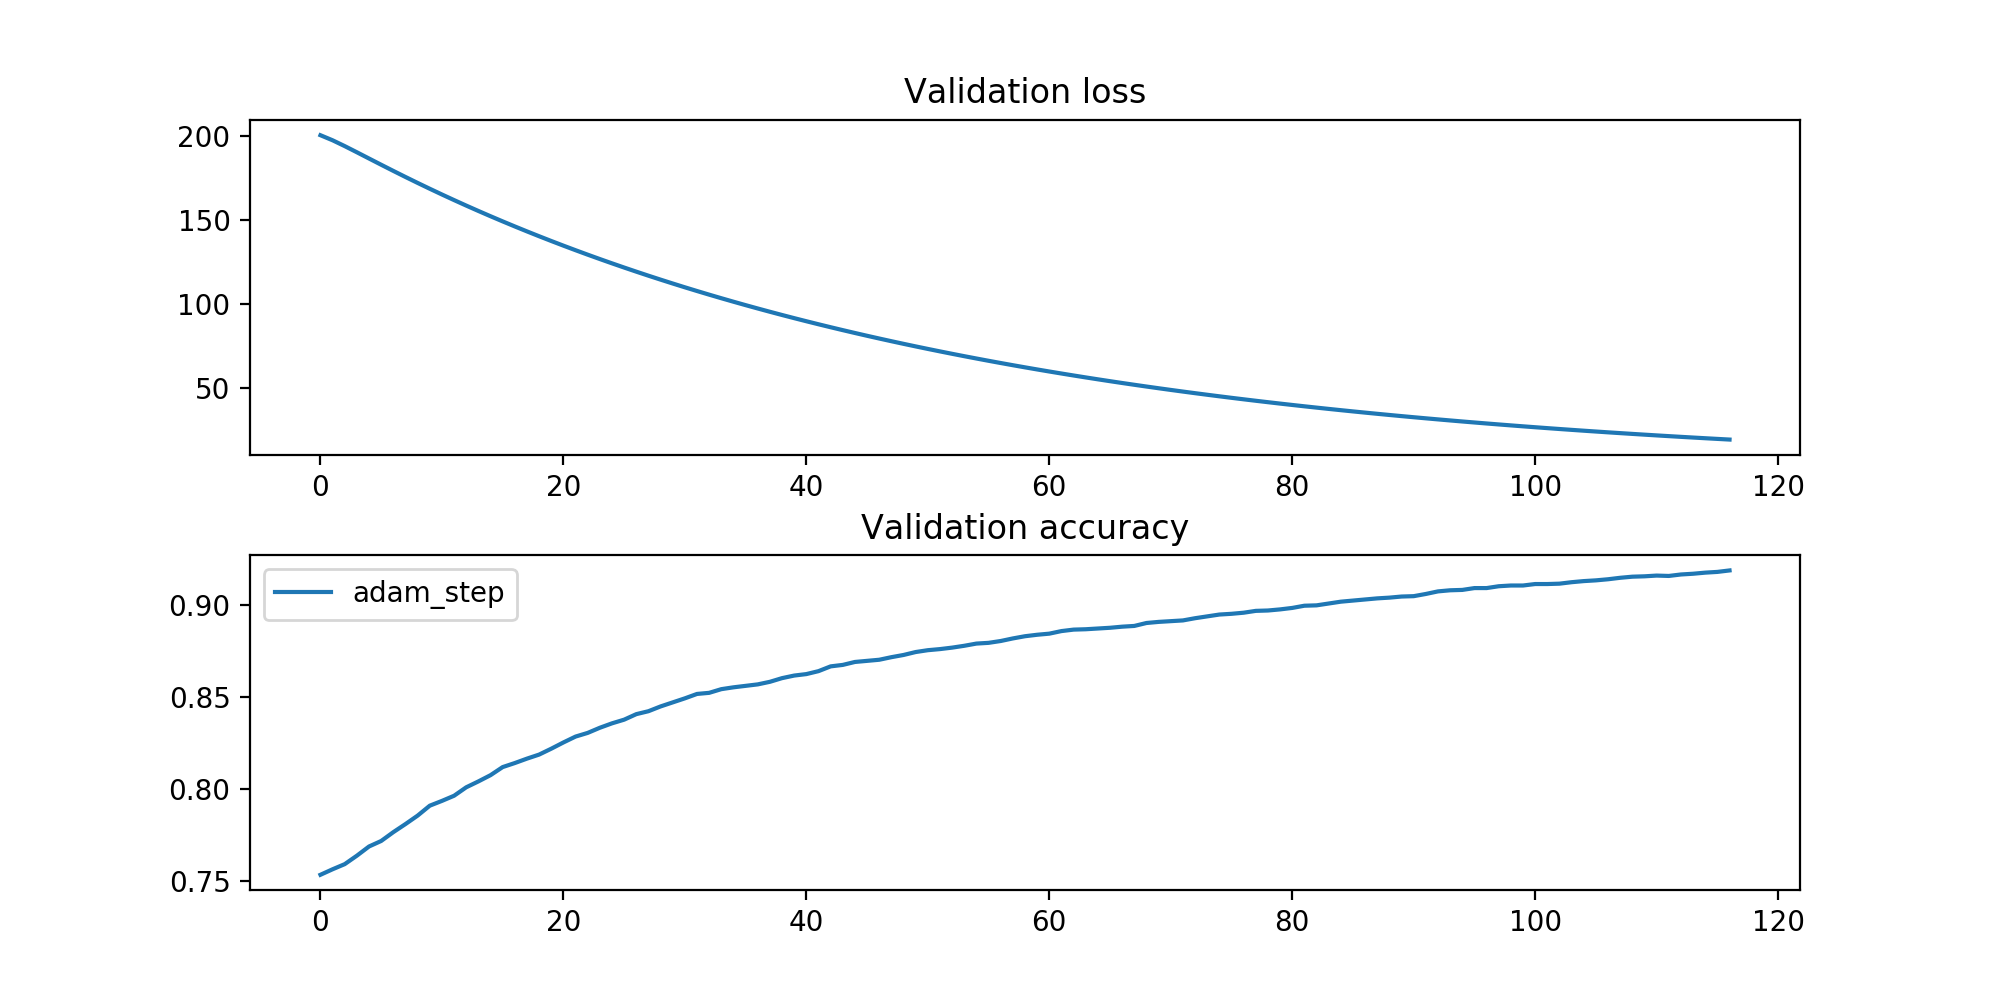
\includegraphics[scale=0.25]{../gdsvm/exports/mnist-batch512-adam_step.png}
			\caption{batch\_size = 512}
		\end{subfigure}
		
		\caption{Influence de la taille des batch sur Adam}
	\end{figure}


			\begin{figure}[H]
	\centering
	\begin{subfigure}{0.45\textwidth}
		\centering
		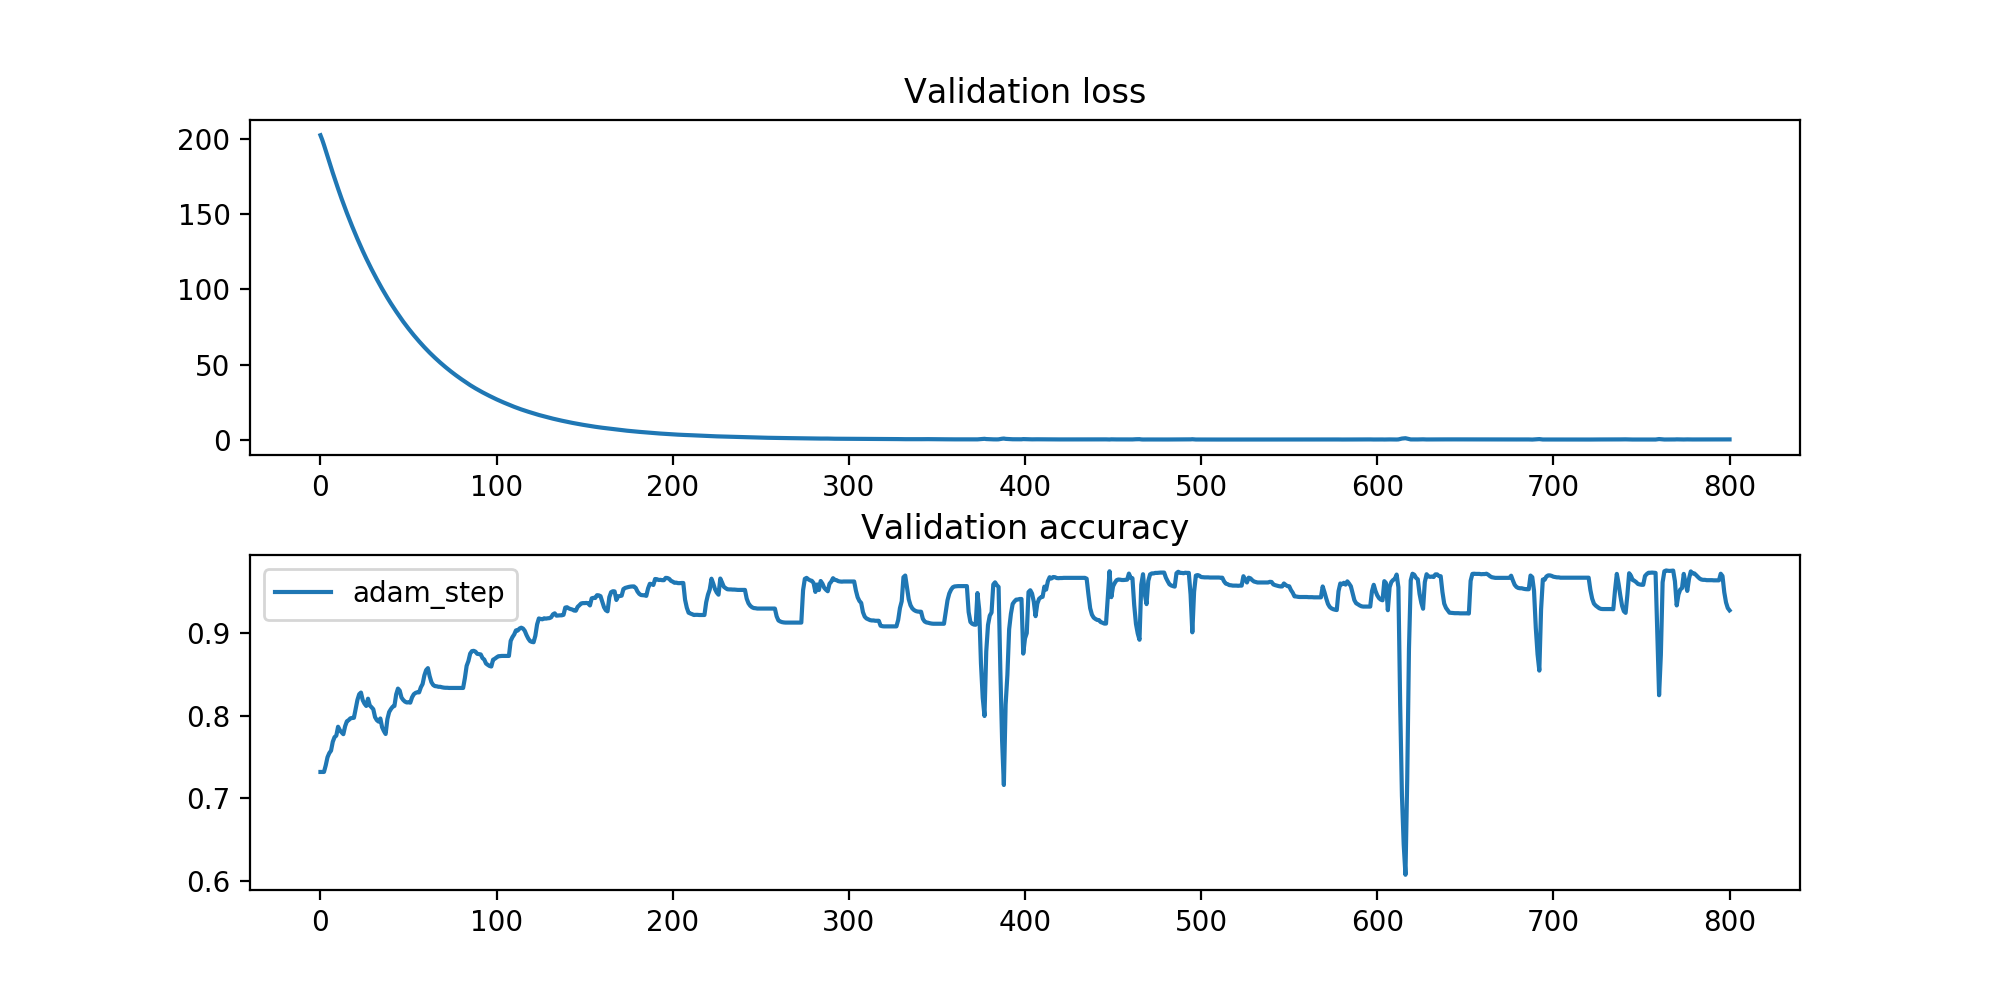
\includegraphics[scale=0.29]{../gdsvm/exports/mnist-batch1-adam_step.png}
		\caption{batch\_size = 1}
	\end{subfigure}
	\begin{subfigure}{0.45\textwidth}
		\centering
		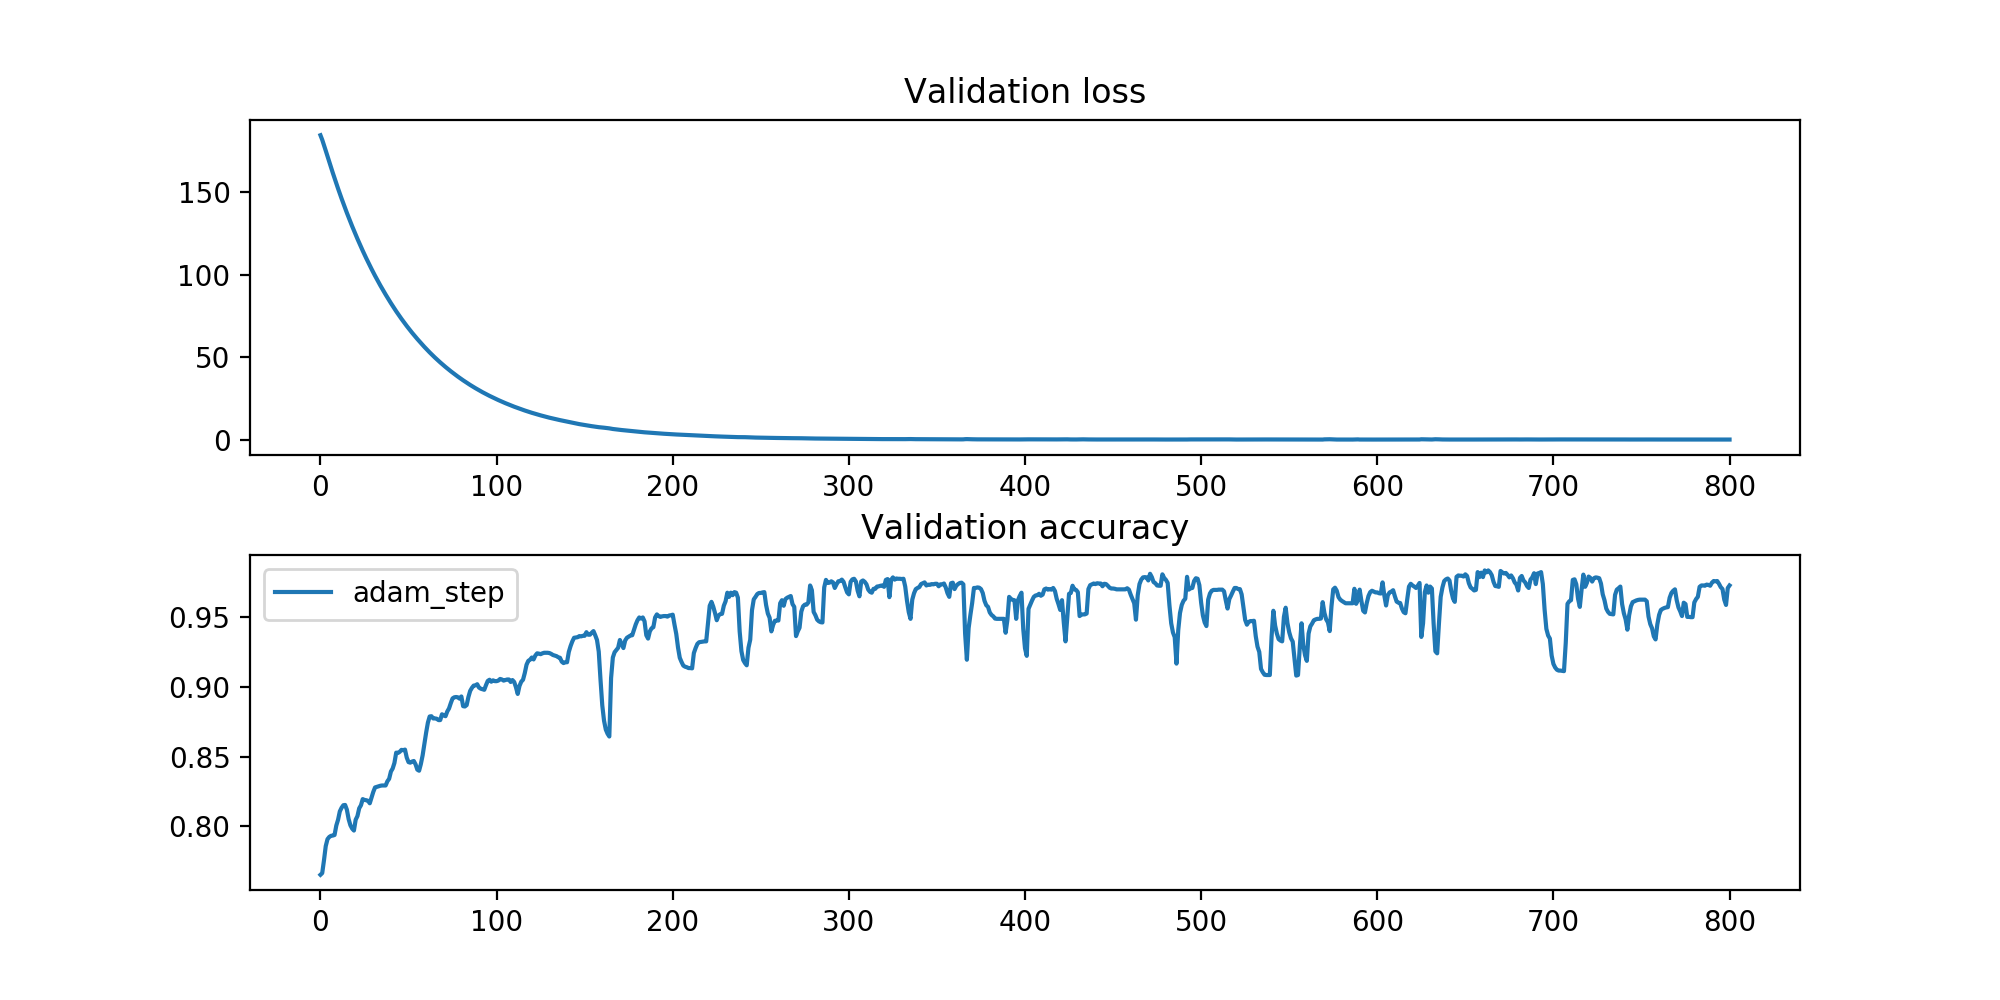
\includegraphics[scale=0.29]{../gdsvm/exports/mnist-batch2-adam_step.png}
		\caption{batch\_size = 2}
	\end{subfigure}
	\begin{subfigure}{1\textwidth}
		\centering
		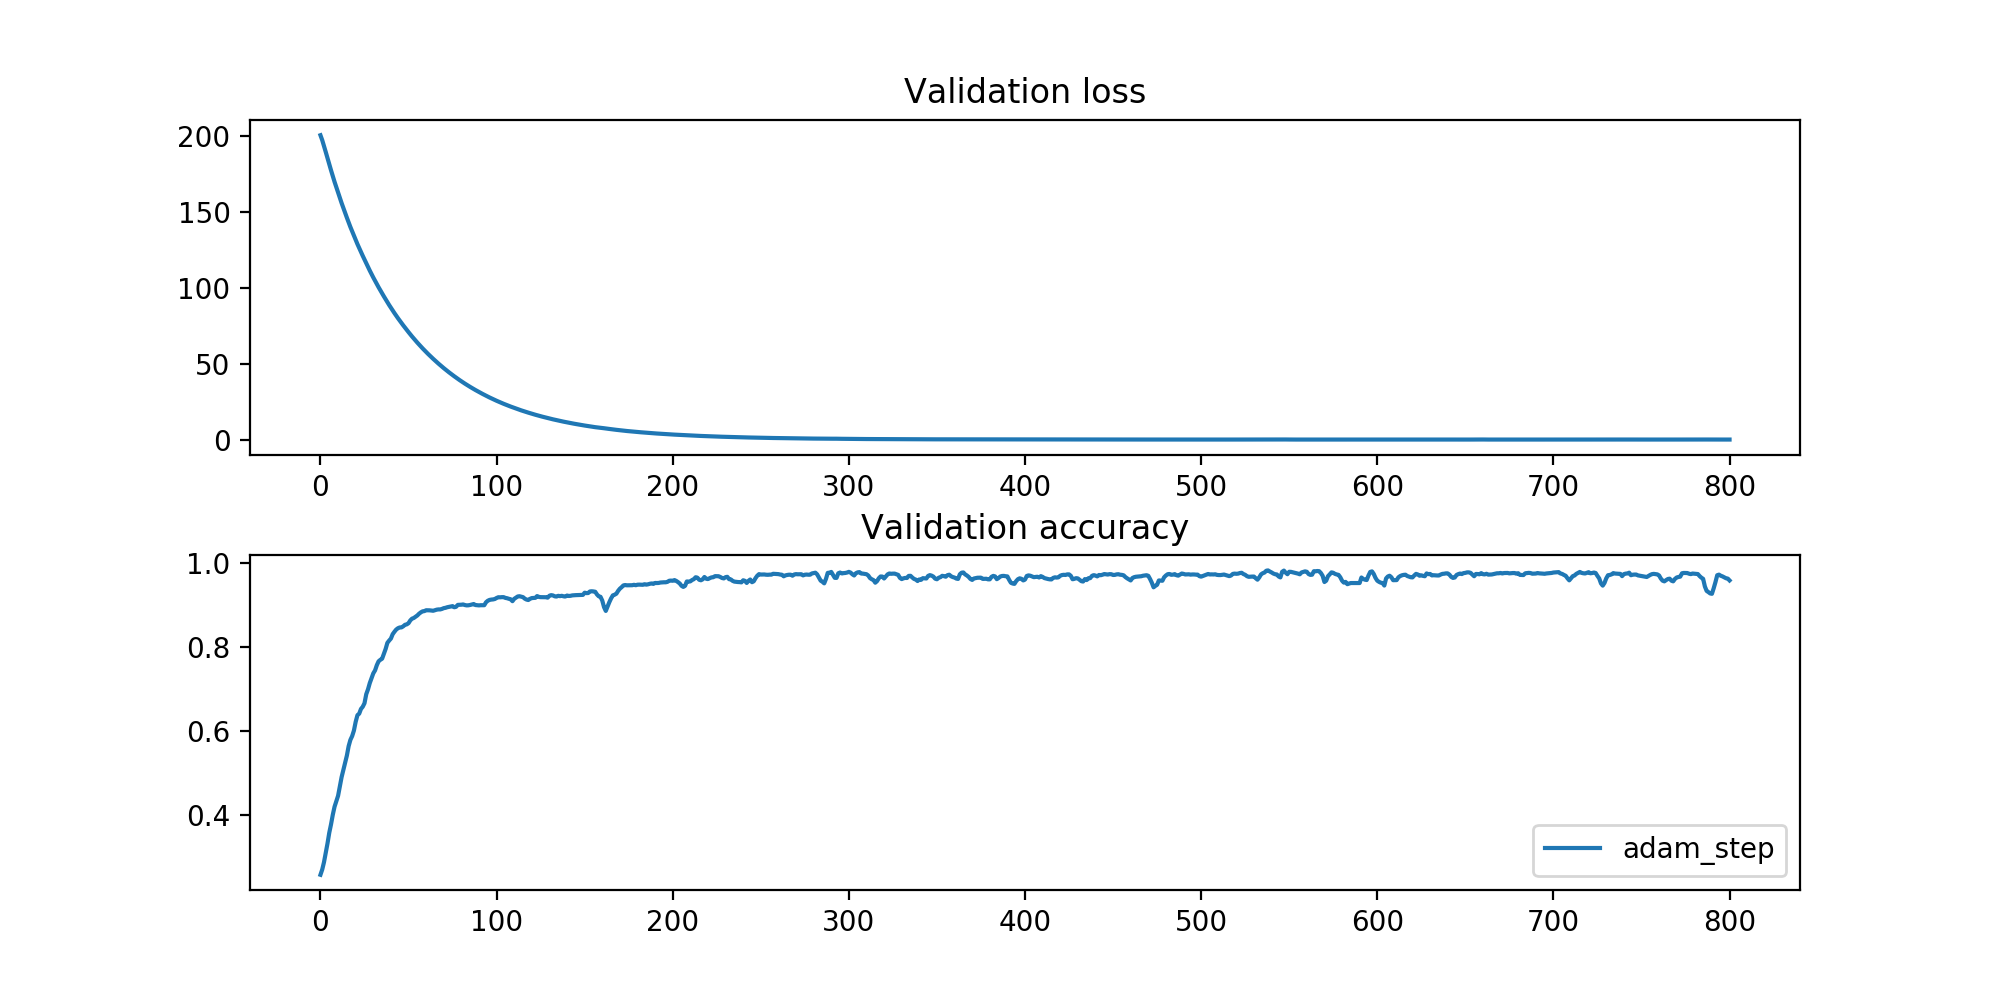
\includegraphics[scale=0.4]{../gdsvm/exports/mnist-batch5-adam_step.png}
		\caption{batch\_size = 5}
	\end{subfigure}
	
	\caption{Influence de la taille des batch sur Adam}
\end{figure}

	Et comparer les résultats avec les autres algorithmes usuels.
	
		
	\begin{figure}[H]
		\centering
		\begin{subfigure}{0.45\textwidth}
			\centering
			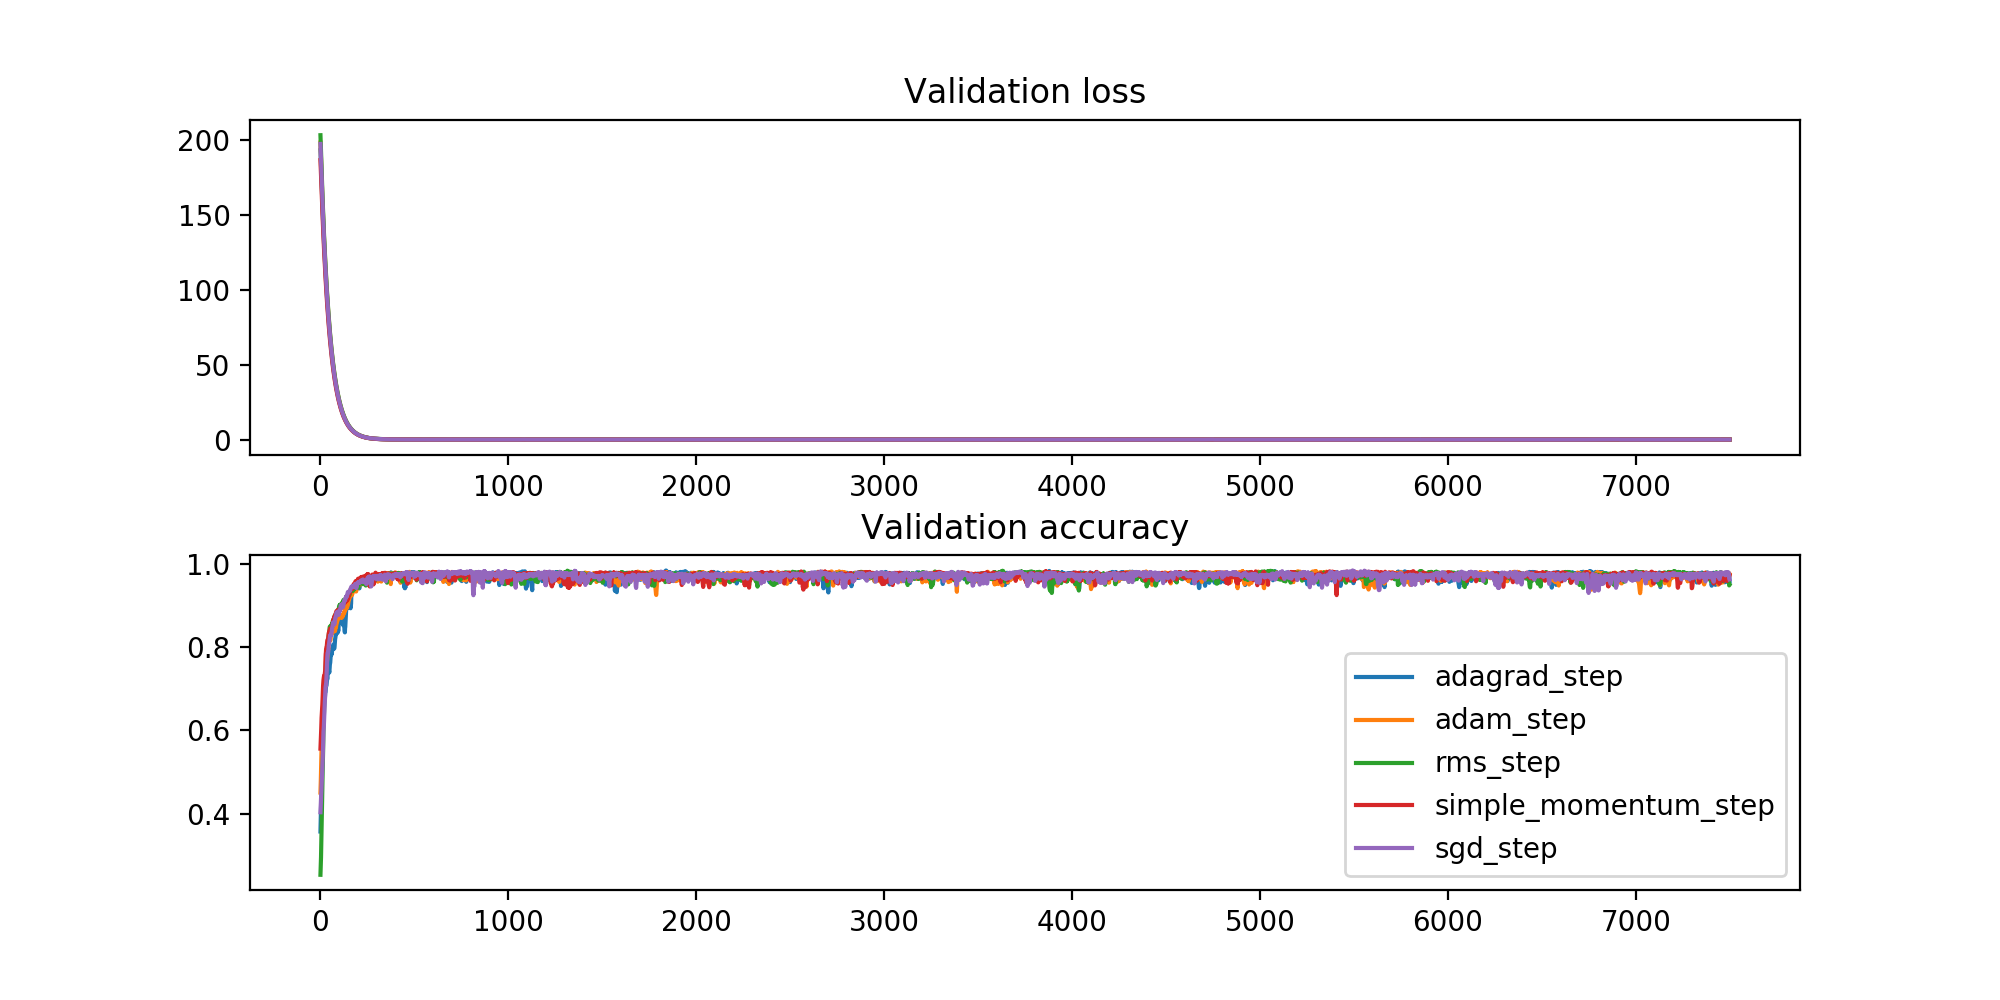
\includegraphics[scale=0.25]{../gdsvm/exports/mnist-batch8-comparison.png}
			\caption{batch\_size = 8}
		\end{subfigure}
		\begin{subfigure}{0.45\textwidth}
			\centering
			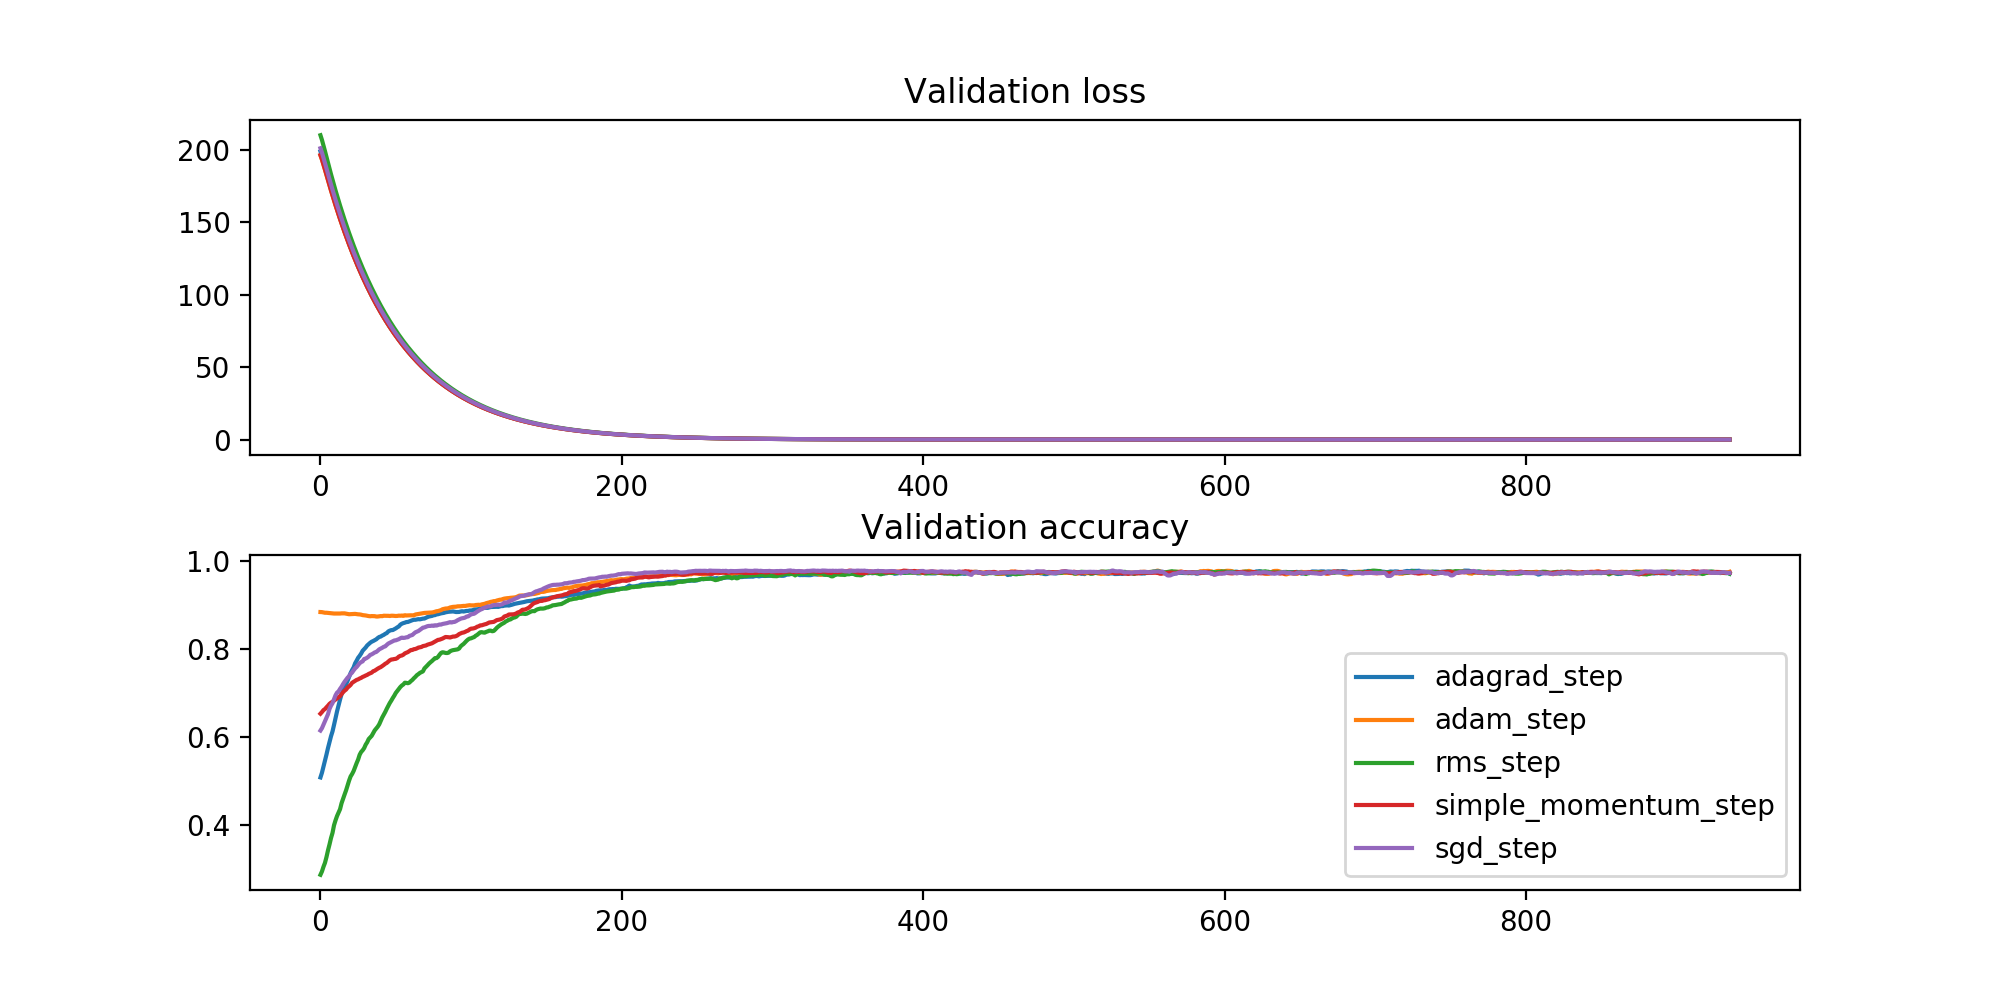
\includegraphics[scale=0.25]{../gdsvm/exports/mnist-batch64-comparison.png}
			\caption{batch\_size = 64}
		\end{subfigure}
		\begin{subfigure}{0.45\textwidth}
			\centering
			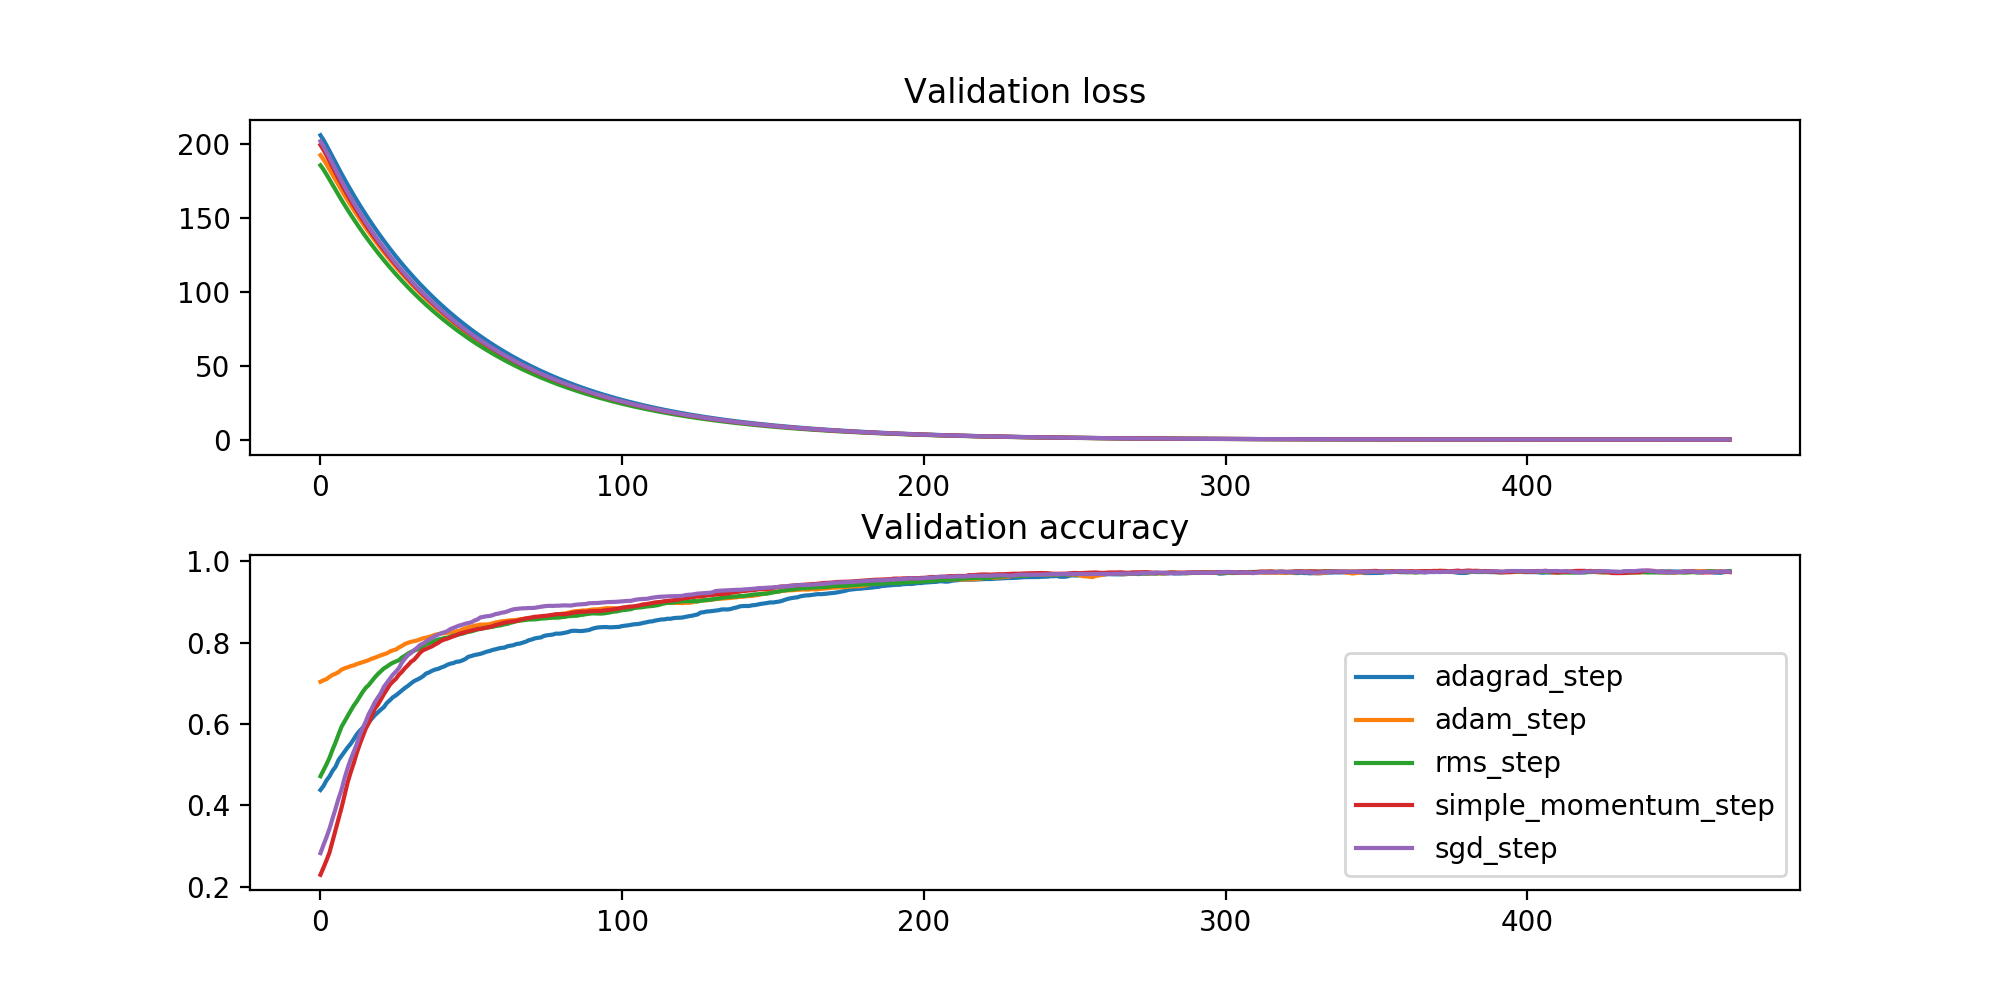
\includegraphics[scale=0.25]{../gdsvm/exports/mnist-batch128-comparison.png}
			\caption{batch\_size = 128}
		\end{subfigure}
		\begin{subfigure}{0.45\textwidth}
			\centering
			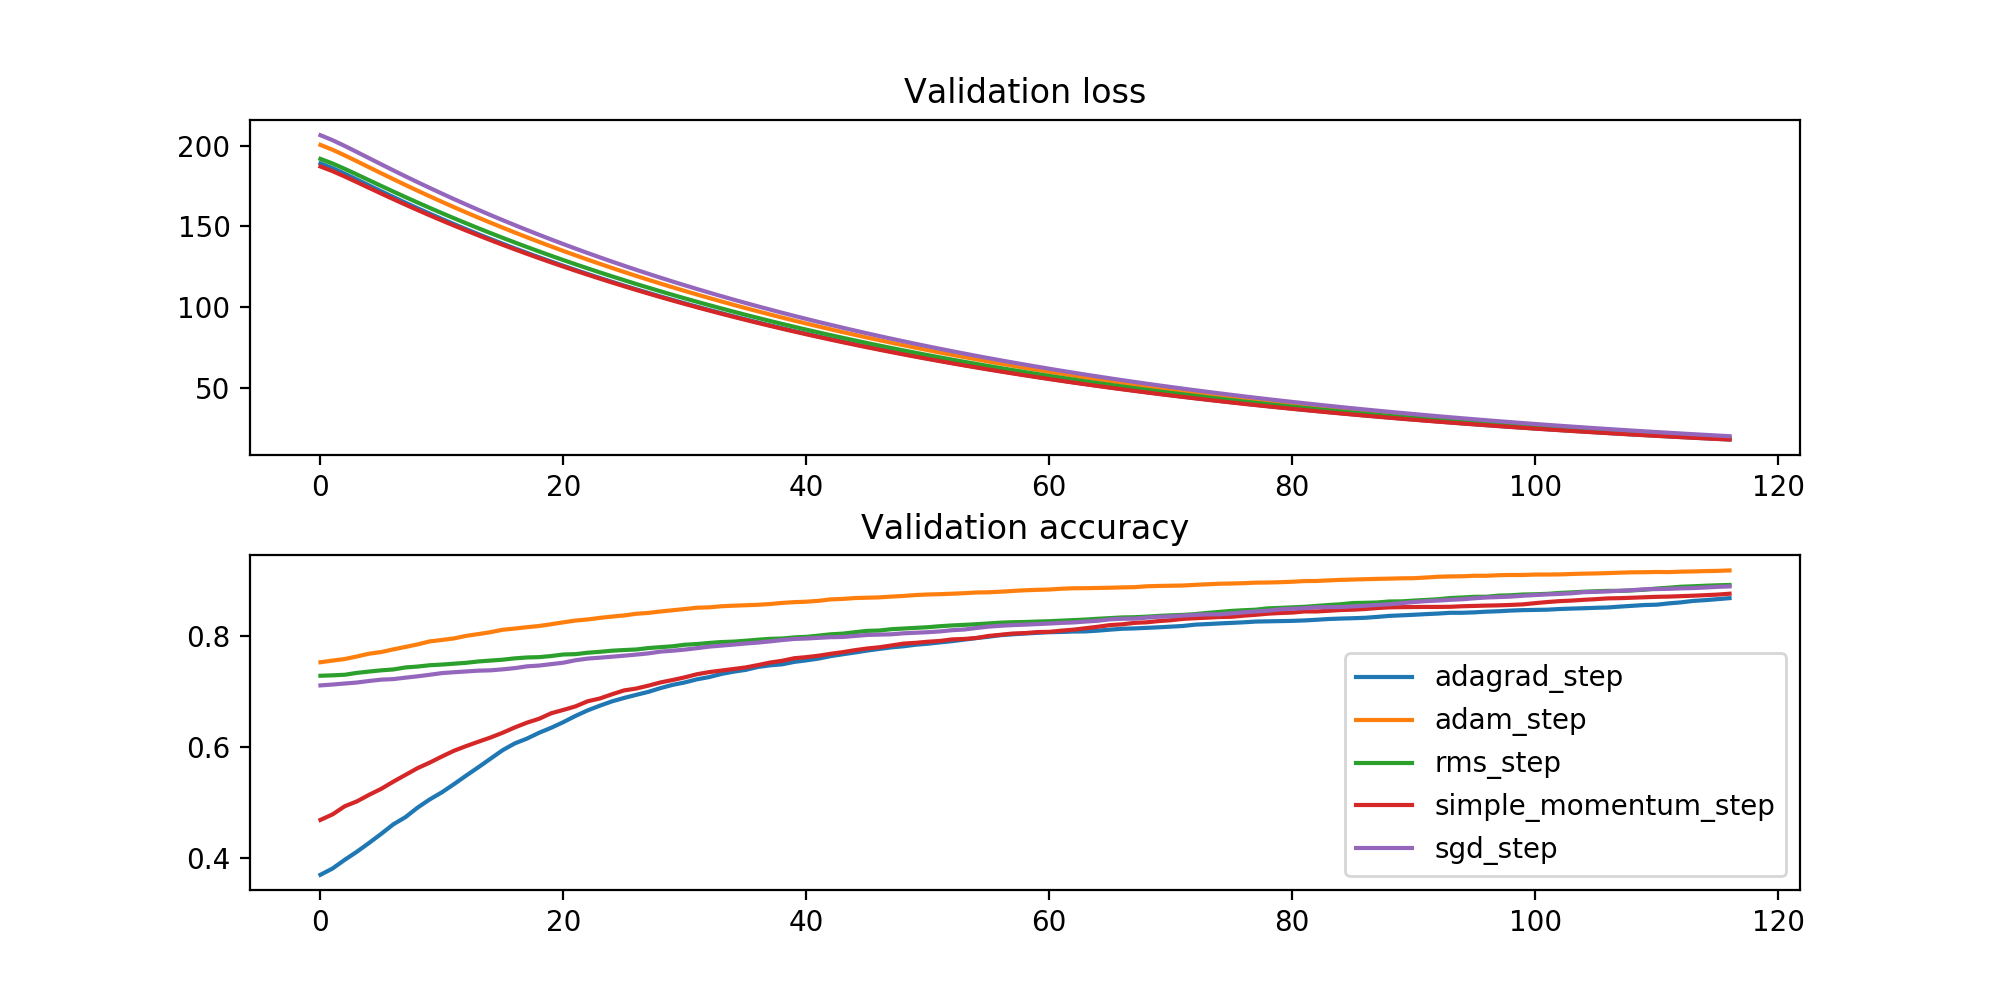
\includegraphics[scale=0.25]{../gdsvm/exports/mnist-batch512-comparison.png}
			\caption{batch\_size = 512}
		\end{subfigure}
		
		\caption{Influence de la taille des batch, comparaison avec les autres algorithmes}
	\end{figure}

	\begin{figure}[H]
	\centering
	\begin{subfigure}{0.45\textwidth}
		\centering
		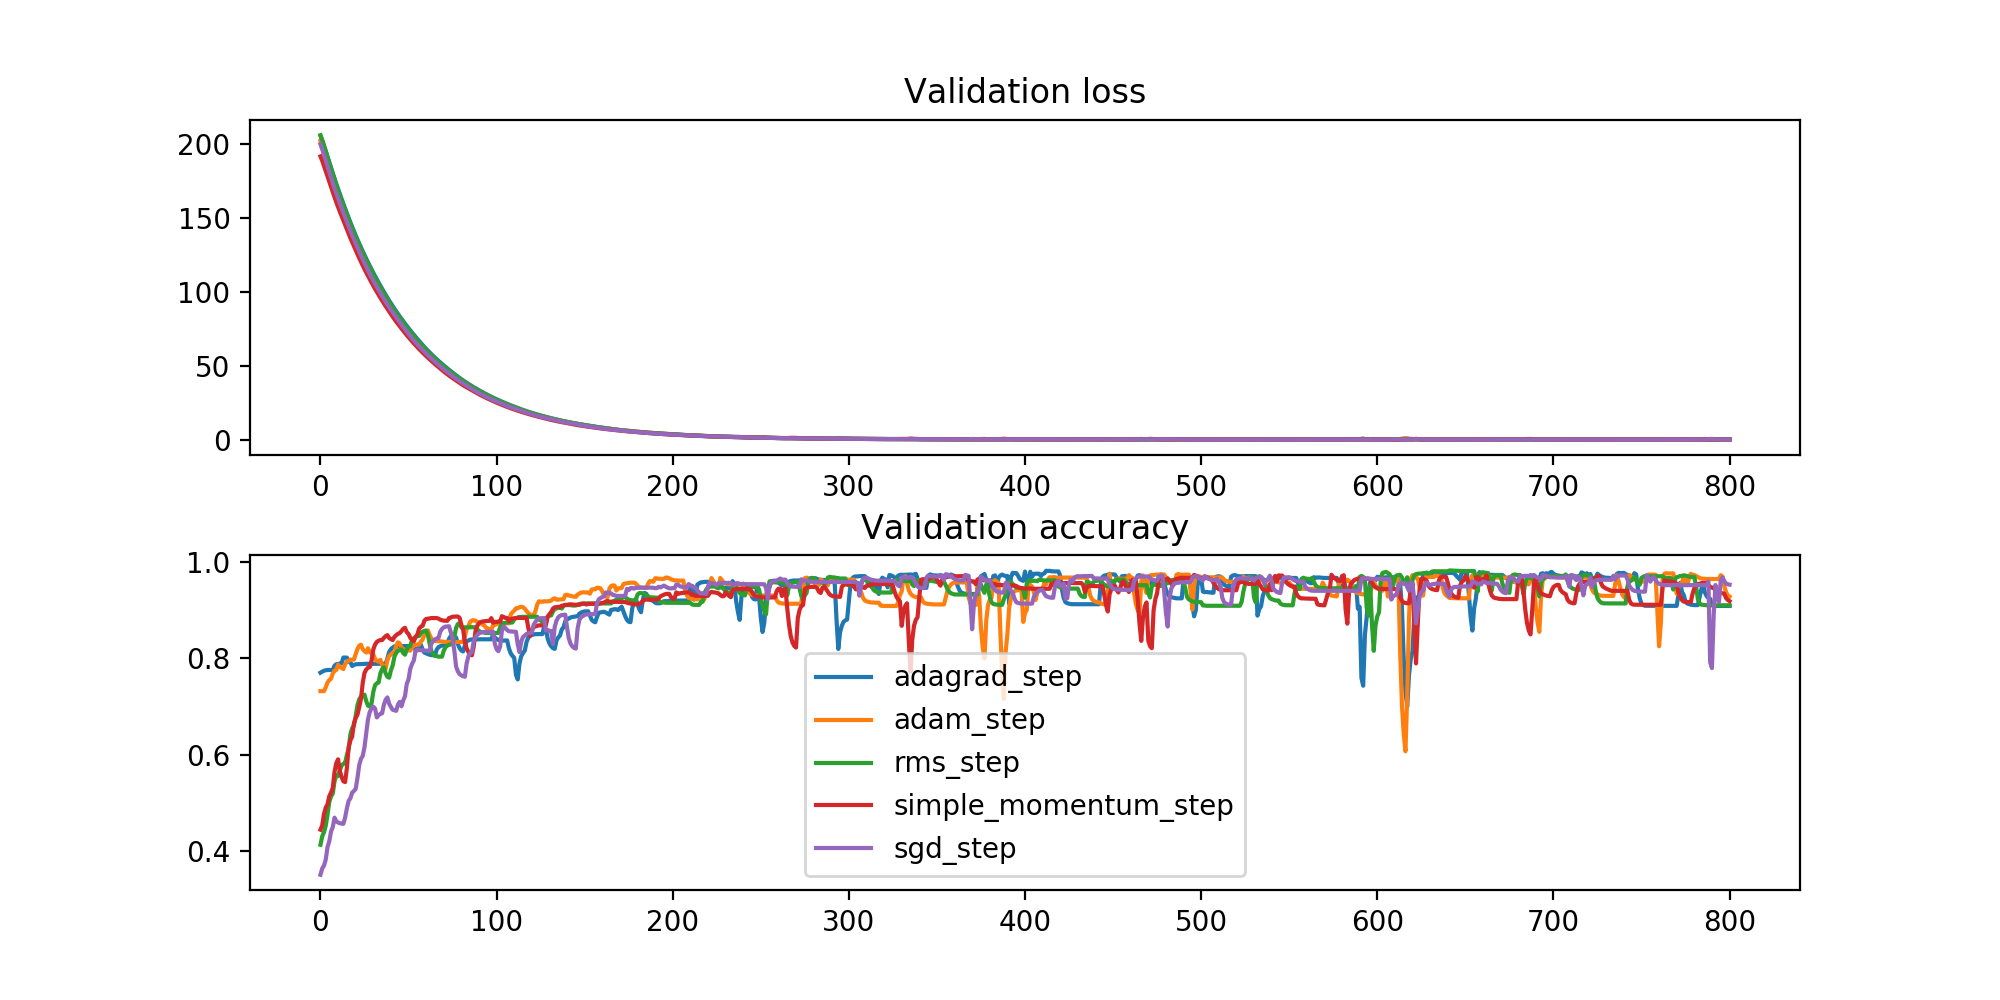
\includegraphics[scale=0.25]{../gdsvm/exports/mnist-batch1-comparison.png}
		\caption{batch\_size = 1}
	\end{subfigure}
	\begin{subfigure}{0.45\textwidth}
		\centering
		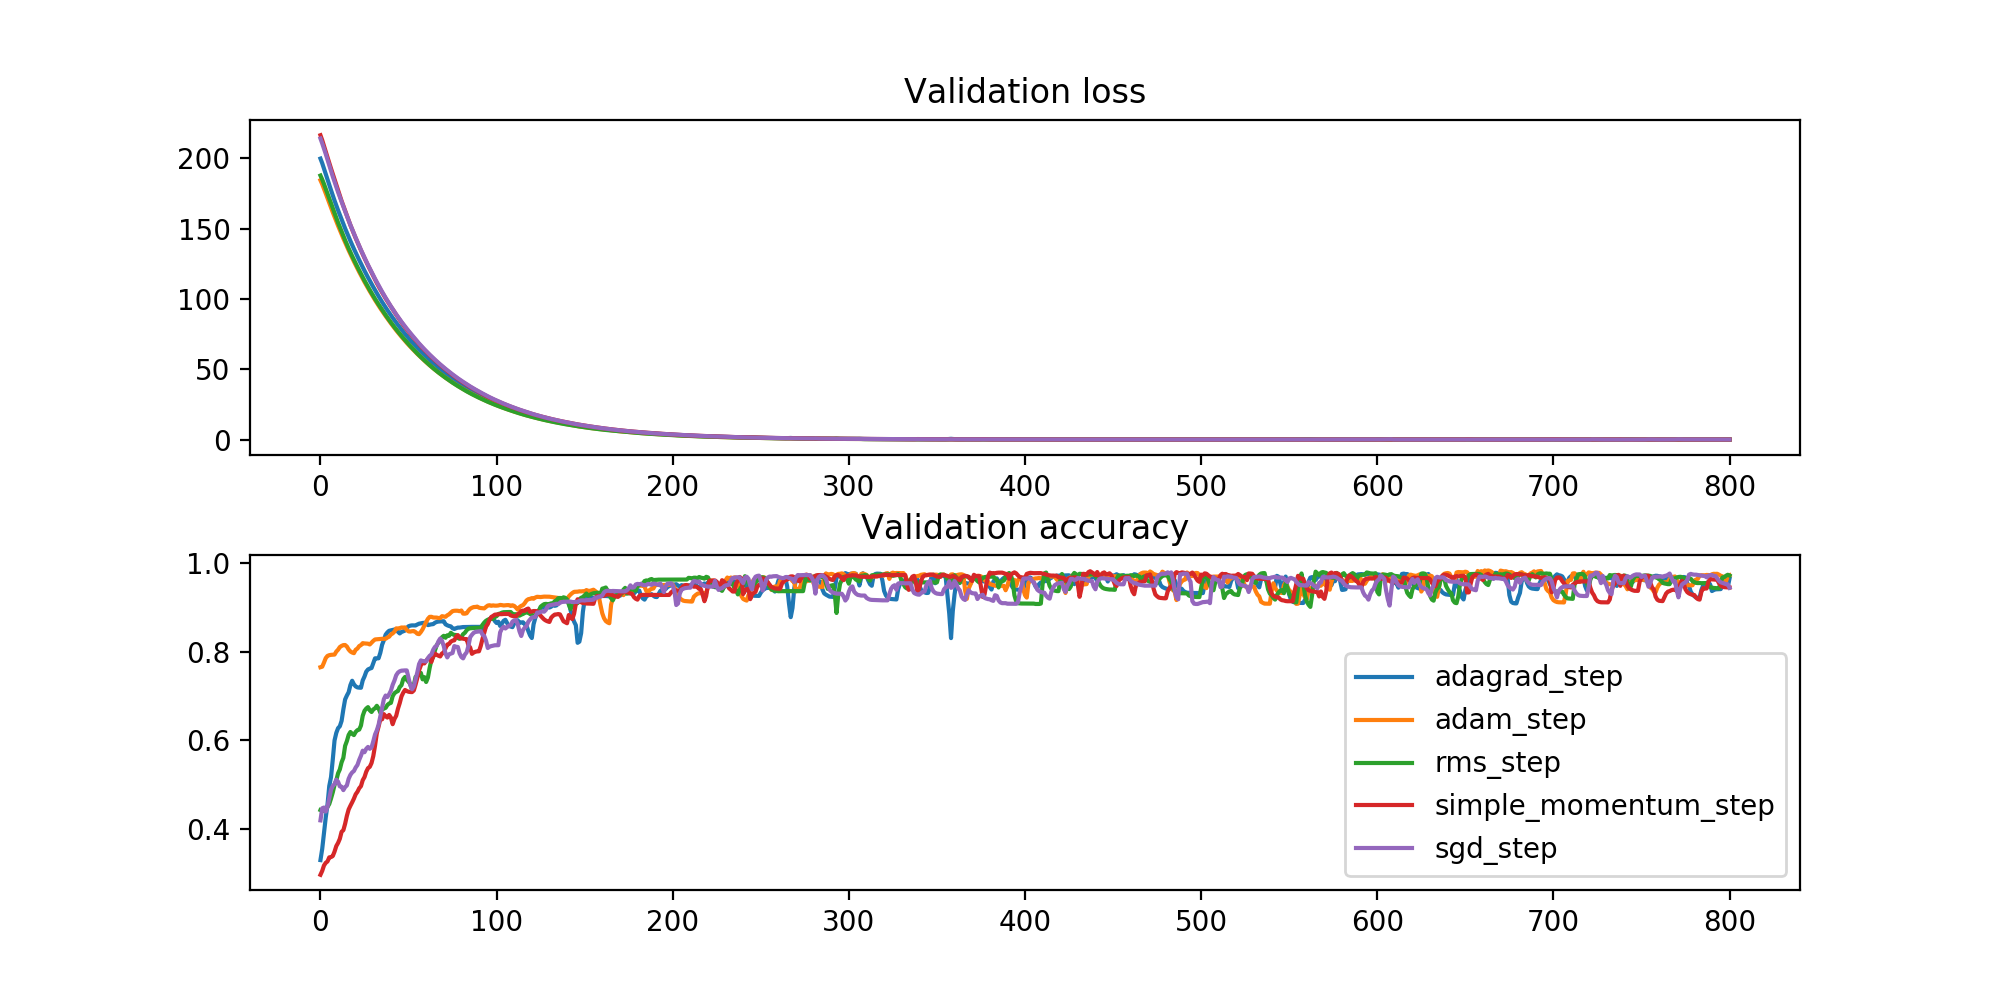
\includegraphics[scale=0.25]{../gdsvm/exports/mnist-batch2-comparison.png}
		\caption{batch\_size = 2}
	\end{subfigure}
	\begin{subfigure}{1\textwidth}
		\centering
		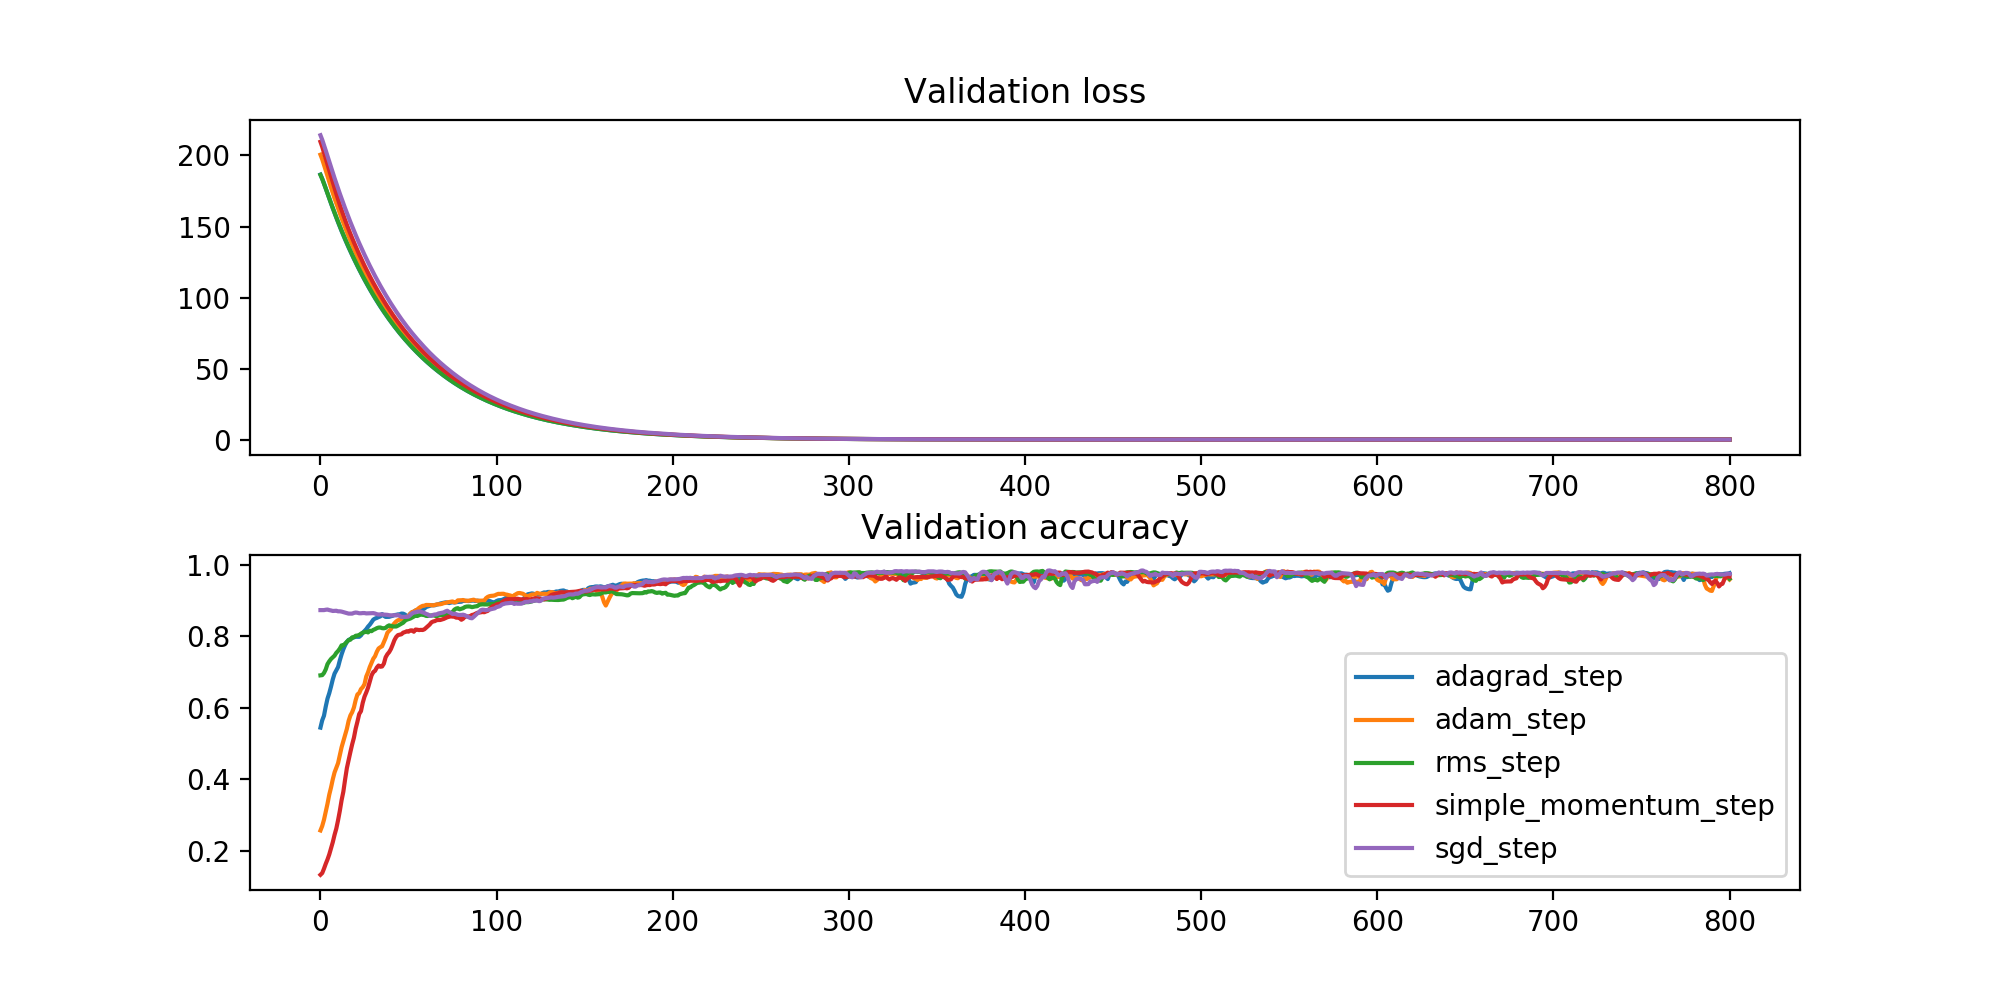
\includegraphics[scale=0.4]{../gdsvm/exports/mnist-batch5-comparison.png}
		\caption{batch\_size = 5}
	\end{subfigure}
	
	\caption{Influence de la taille des batch, comparaison avec les autres algorithmes}
\end{figure}

	On peut noter la vitesse de convergence bien plus grande de \emph{Adam} sur les grands batch que pour les autres algorithmes.
	
\bibliographystyle{plain}	
\bibliography{biblio}

	

	
	

	
	

\end{document}
